\chapter{Referencial Teórico}
\label{cap:referencial-teorico}

Nesta seção serão apresentados os assuntos fundamentais para o entendimento dos processos envolvidos no uso das tecnologias abordadas no decorrer do trabalho. No início será discutida a criação dos \textit{shaders} e seu uso ao longo do tempo, em seguida serão expostos itens de ordem técnica sobre os \textit{shaders} e os motores de jogo. Ao final será tratada a integração dessas tecnologias com os processos de otimização.

\section{Evolução da Programação de Shaders}
\label{sec:historia-evolucao-programacao-shaders}

As representações visuais feitas através de imagens são até hoje uma característica importante da formação da humanidade. Através do sentido da visão conseguimos absorver informações rapidamente, fazer associações durante o aprendizado e o estudo, ou ainda distinguir se algo é visualmente agradável o suficiente ou não para prender nossa atenção (LUTEN, 2021)\nocite{openGLBook}.

O acesso aos primeiros computadores era restrito devido aos custos elevados e a logística complexa. A representação visual dos pulsos elétricos gerados pelo seu processamento de dados era feita através de várias lâmpadas conectadas em placas ou de cartões de papel perfurados. Esse cenário começou a mudar depois da aplicação da tecnologia do tubo de raios catódicos (\acrshort{CRT}), em 1951, pelo Instituto de Tecnologia de Massachusetts (MIT) para visualizar a saída de um programa instantaneamente (LUTEN, 2021)\nocite{openGLBook}.

O estabelecimento da computação gráfica teve início 10 anos depois. A partir da criação de um programa de computador por Ivan Sutherland chamado \textit{Sketchpad}, que permitia desenhar formas geométricas utilizando uma caneta óptica em um \acrshort{CRT} com visualização em tempo real (LUTEN, 2021)\nocite{openGLBook}. Isso causou uma mudança de padrão na forma como as pessoas entendiam e utilizavam os computadores e foi o ponto de partida para desenvolvimento da computação gráfica em tempo real.
	
Com a criação dos circuitos integrados a indústria de microprocessadores sofreu um crescimento enorme. Os computadores deixaram de ser um monopólio das grandes companhias e tornaram-se mais acessíveis a pessoas simples. Isso abriu várias possibilidades para o mercado de computadores pessoais, entre elas destaca-se o surgimento das primeiras placas gráficas produzidas pela \acrlong{IBM} (IBM).   
	
Com as melhorias de \textit{hardware} disponíveis, a indústria de jogos eletrônicos tinha mais recursos para explorar. Os casos mais marcantes, mostrados na Figura \ref{fig:exemplo-3}, se deram pela empresa \textit{id Software} na década de 90. O primeiro sendo Wolfenstein 3D --- que na realidade utilizava o modo 7 do Super NES (\acrlong{NES}) para emular a ambientação tridimensional --- e o segundo sendo Doom que fazia uso de renderização com perspectiva 3D em tempo real por meio de \textit{software} desenvolvido pela própria \textit{id Software}.
	
    \begin{figure}[h]
		\centering
		\Caption{\label{fig:exemplo-3} Doom faz uso de 3D (esquerda) enquanto Wolfenstein posiciona imagens em diferentes camadas para simular a profundidade (direita).}	
		\UNIFORfig{}{
			\fbox{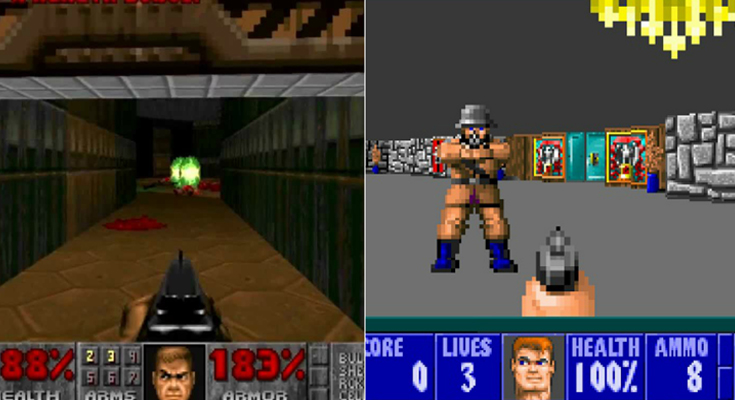
\includegraphics[width=11cm]{figuras/figura-3}}
		}{
			\Fonte{Retro Refurbs (2021)}
		}
	\end{figure}
	\nocite{figura3}
	
Paralelamente, a Silicon Graphics (\acrshort{SGI}) --- companhia especializada em computação gráfica 3D --- trabalhava no lançamento da Open Graphics Library (\acrshort{OpenGL}), uma \acrlong{API} (API) \textit{open source} padronizada multiplataforma de processamento de gráficos de computador em tempo real derivada de outra biblioteca proprietária da mesma empresa, a IRIS GL (\acrlong{IRIS GL}) e que rapidamente dominou o mercado (LUTEN, 2021)\nocite{openGLBook}. 

A Microsoft, para competir, comprou a empresa RenderMorphics, criadora da \acrshort{API} Reality Lab, que teve o nome alterado para Direct3D e foi distribuido como um SDK (\acrlong{SDK}) conhecido como DirectX, que acabou sendo o concorrente direto da \acrshort{OpenGL} (LUTEN, 2021)\nocite{openGLBook}. Essa rivalidade acabou sendo benéfica tanto para o mercado de jogos eletrônicos quanto para os seus consumidores, já que acelerou o desenvolvimento de tecnologias que exploravam ao máximo o potencial do \textit{hardware} disponível.
	
 	\begin{figure}[h!]
		\centering
        \Caption{\label{fig:1} \textit{Hardware} da placa gráfica da NVIDIA.}
        \begin{subfigure}{0.45\textwidth}
        \UNIFORfig{}{
			\fbox{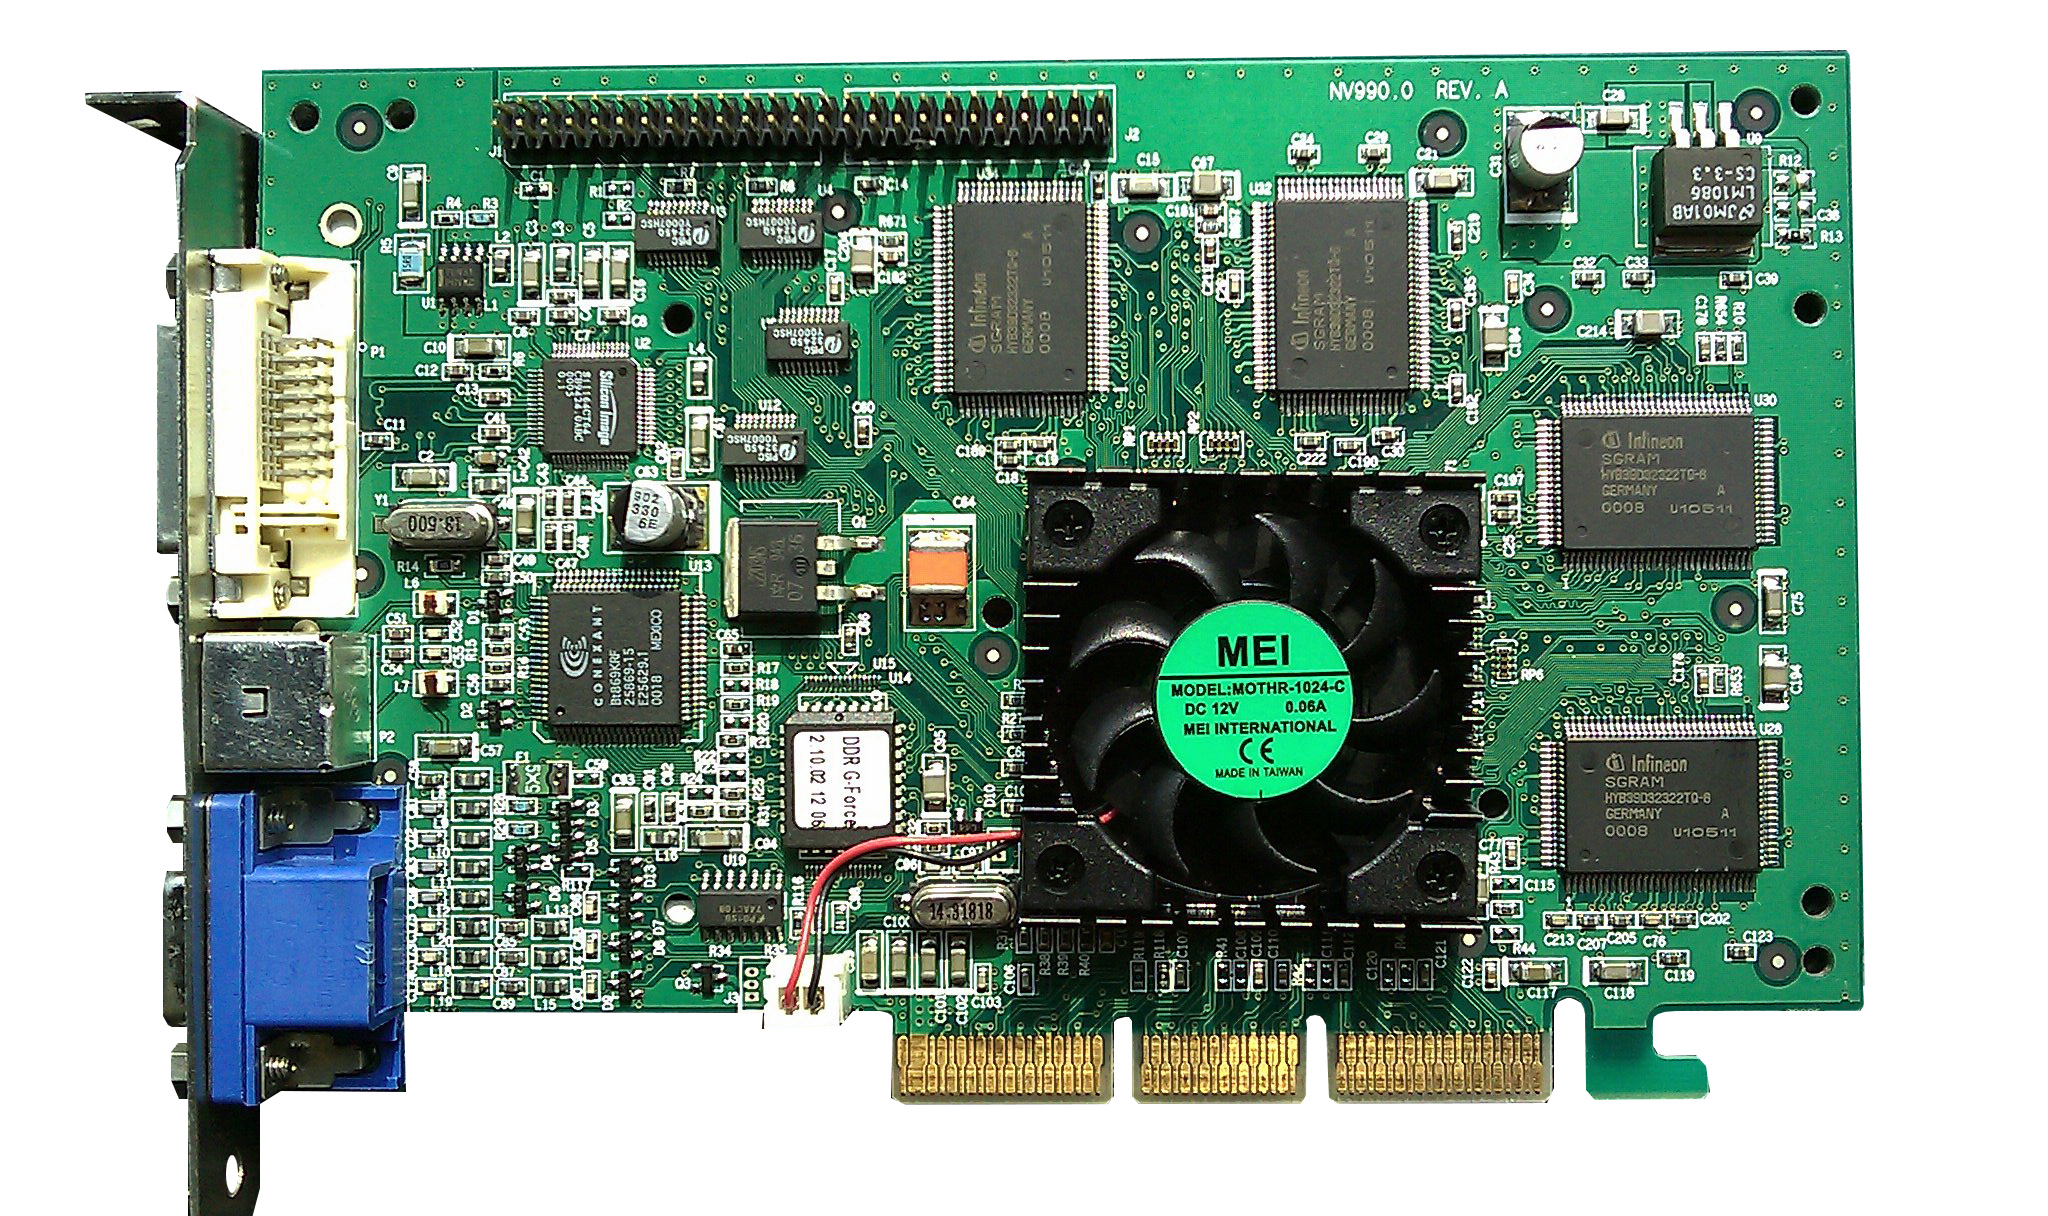
\includegraphics[width=\linewidth]{figuras/fig-a}}
		}{
		    \caption{GeForce 256} \label{fig:1a}
		}
		\nocite{figura4a}
        \end{subfigure}%
        
        \begin{subfigure}{0.25\textwidth}
        \UNIFORfig{}{
			\fbox{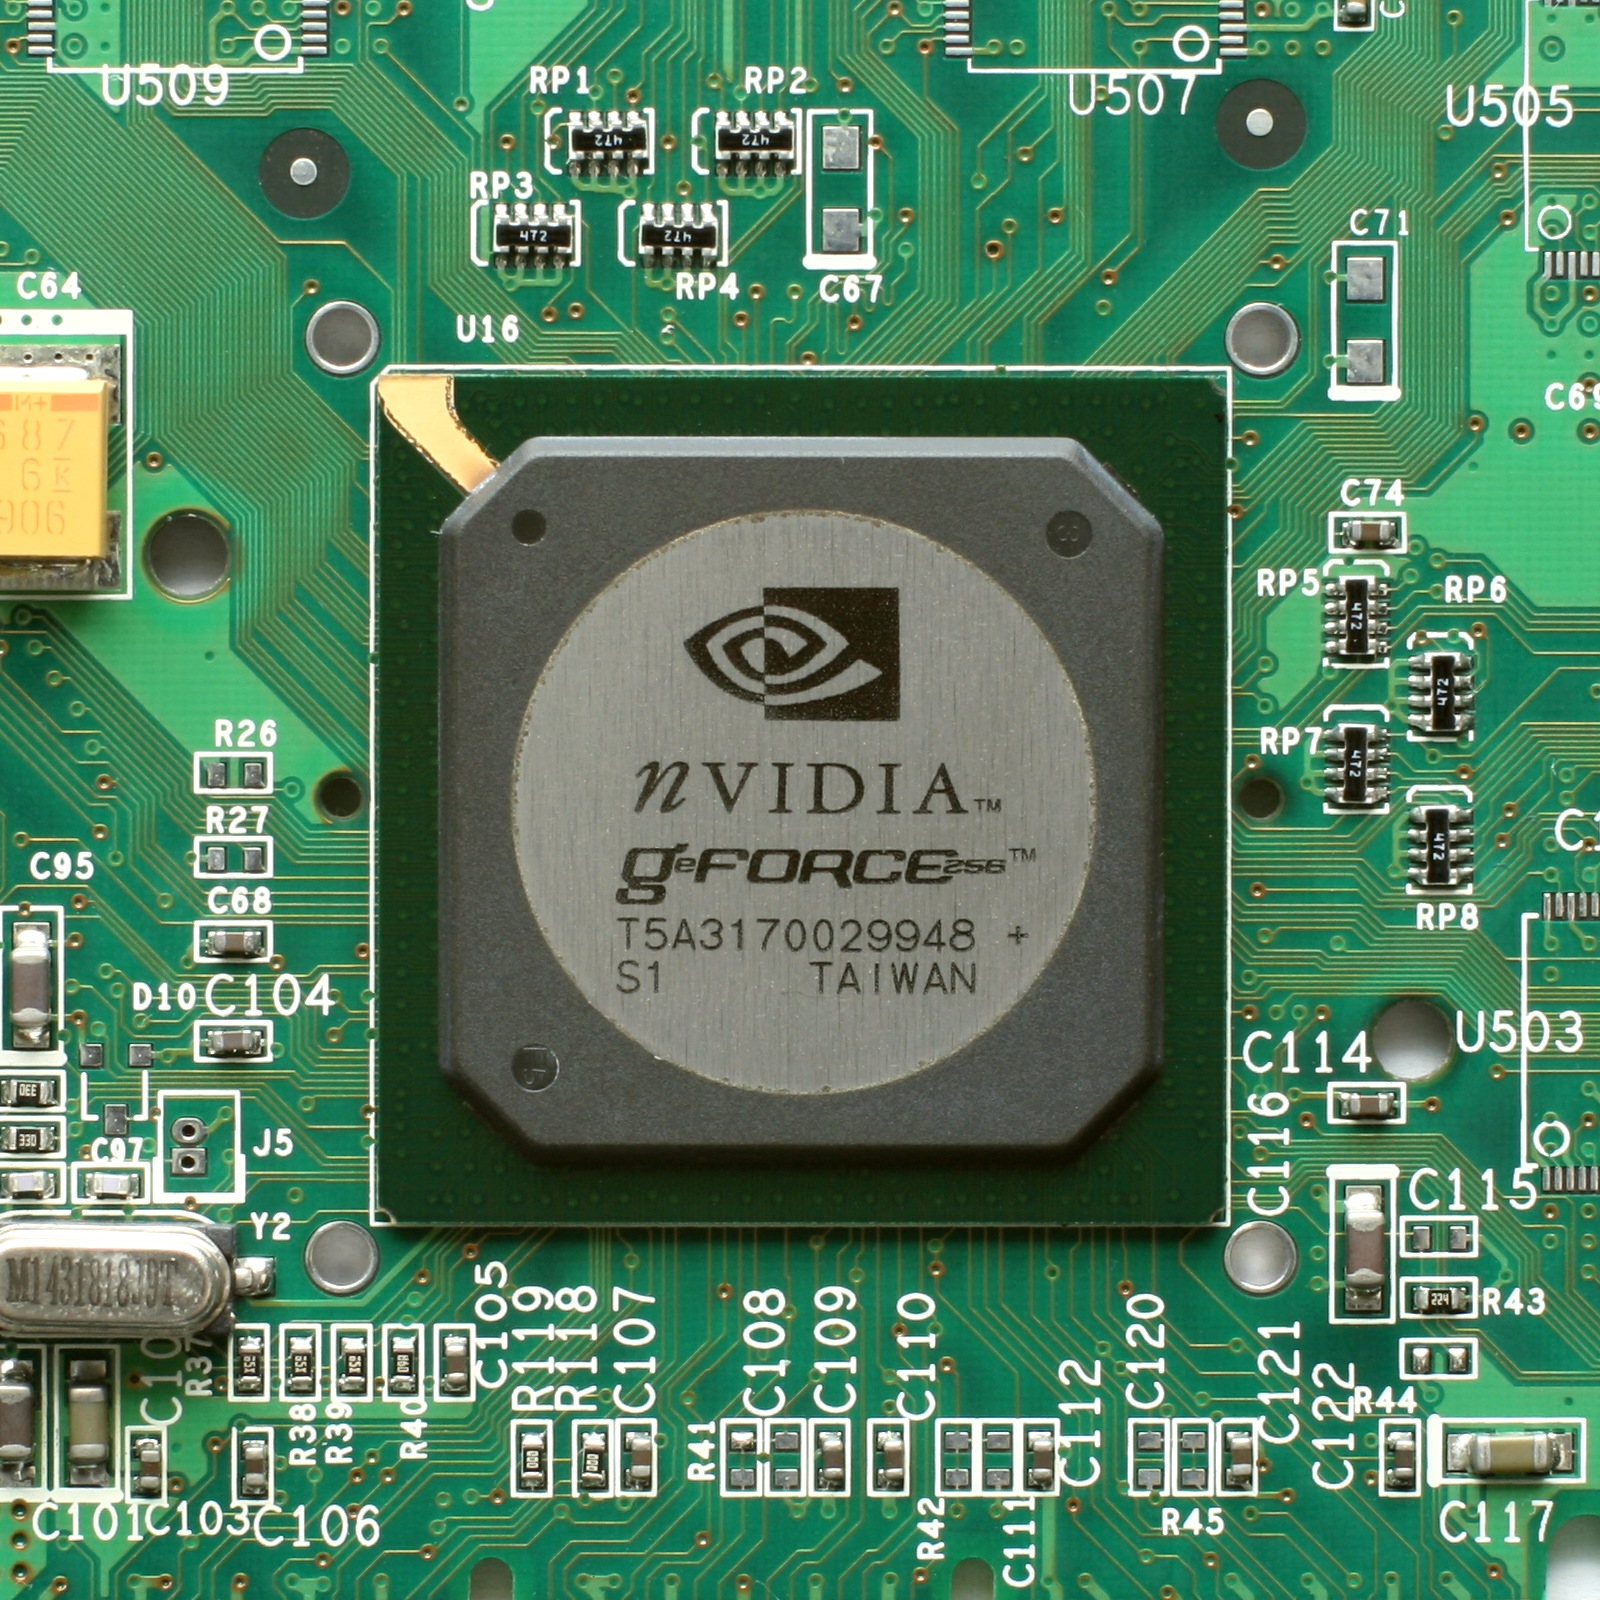
\includegraphics[width=\linewidth]{figuras/fig-b}}
		}{
		    \caption{GPU da GeForce 256} \label{fig:1b}
		}
		\nocite{figura4b}
        \end{subfigure}
		{
			\Fonte{Wikimedia (2021)}
		}
	\end{figure}

Em 1999, a empresa NVIDIA lançou a placa gráfica GeForce 256 (Figura \ref{fig:1}), que possuia a tecnologia T\&L (\acrlong{T+L}) que movia os cálculos de transformação e iluminação de vértices da CPU (\acrlong{CPU}) para a \acrshort{GPU} (\acrlong{GPU}), aumentando a velocidade em operações matemáticas de ponto flutuante. Nos anos seguintes houve um crescimento exponencial de performance de \acrshort{GPU}.

Uma GPU é um circuito eletrônico projetado para realizar manipulações rápidas em memória para acelerar a criação de imagens em um \textit{buffer} de quadros que envia a saída para uma tela. Em aplicações que exigem muitas operações vetoriais, o poder de computação paralelo da GPU consegue entregar maior performance que uma CPU convencional. Daí seu vasto uso em jogos eletrônicos, mas também em outras áreas, principalmente na ciência \cite{shea2013gpu}.

Até então \textit{shaders} eram bastante utilizados por melhorar a performance eliminando carga de trabalho excessiva da \acrshort{CPU}, porém sua programação era difícil devido a sintaxe utilizada ser semelhante à programação em Assembly. A Microsoft então lançou a versão 9.0 do Direct3D que trazia \acrlong{HLSL} (HLSL) que permitia a programação de \textit{shaders} em alto nível e possuia uma sintaxe bastante parecida com C (LUTEN, 2021)\nocite{openGLBook}. Enquanto isso, OpenGL também trouxe a sua própria linguagem de alto nível chamada \acrlong{GLSL} (GLSL). 

\subsection{Como o OpenGL funciona}
\label{sec:como-opengl-funciona}

Para Rost (2006), a API do OpenGL desenha gráficos em uma memória especializada em quadros de imagem (\textit{frame buffer}). Ela oferece suporte tanto a geometrias 3D quanto a imagens simples. O modelo de funcionamento dessa API pode ser descrito como cliente-servidor, pois a aplicação (cliente) faz solicitações por meio de comandos que são interpretados e processados pela implementação OpenGL (servidor). É importante destacar que a sincronia entre cliente e servidor e suas informações/dados não ocorre quando um comando é executado mas sim quando ele é emitido.

Os comandos são sempre processados na ordem em que são recebidos pelo servidor (execução fora de ordem não é permitida). Os dados passados para um comando OpenGL são interpretados e copiados em memória caso seja necessário e as modificações subsequentes feitas pela aplicação não surtem efeito nos dados que estão armazenados internamente pelo OpenGL. Esses procedimentos são uma forma de garantir que um primitivo --- segundo Abdala (2021)\nocite{abdala}, uma representação discreta em grade de um elemento geométrico fundamental, e.g. ponto, linha, círculo, etc --- seja desenhado apenas se o primitivo anterior houver sido completamente desenhado \cite{GLSLBook}.

O principio de funcionamento dessa API é transformar dados vindos de uma aplicação em algo visível na tela, esse processo é chamado de renderização e normalmente é acelerado por \textit{hardware} com design específico (acelerador gráfico), porém suas operações podem ser parcial ou totalmente implementadas por \textit{software} executado pela CPU. Em um sistema de janelas, a janela que corresponde a região da memória gráfica que é modificada durante a renderização é chamada de \textit{frame} \textit{buffer}. Já em um cenário sem janelas (i.e. tela cheia) o \textit{frame} \textit{buffer} corresponde a toda a tela \cite{GLSLBook}.

Para que uma janela suporte a renderização ela precisa de alguns elementos: até quatro \textit{buffers} para as cores, um \textit{buffer} de profundidade (Figura \ref{fig:exemplo-6}), um \textit{stencil buffer} (Figura \ref{fig:exemplo-7}), um \textit{buffer} de acumulação, um \textit{multisample buffer} e um ou mais \textit{buffers} auxiliares. A maioria dos \textit{hardwares} suporta o carregamento duplo, técnica que faz uso de um \textit{buffer} frontal e um \textit{buffer} posterior para que o processo de renderização seja realizado em plano de fundo e então quando terminar seu conteúdo é trocado com o do \textit{buffer} frontal para exibir o resultado final e iniciar a nova renderização. 

\phantom{a}

\phantom{a}

\begin{figure}[h!]
	\centering
	\Caption{\label{fig:exemplo-6} No \textit{buffer} de profundidade objetos próximos ficam com tonalidade mais escura enquanto objetos distantes assumem uma tonalidade mais clara.}	
	\UNIFORfig{}{
		\fbox{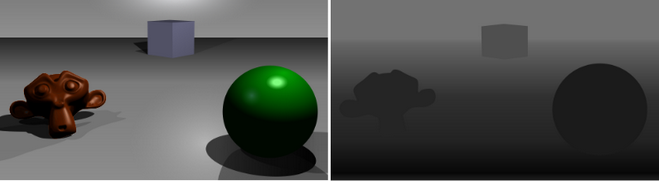
\includegraphics[width=14cm]{figuras/figura-6}}
	}{
		\Fonte{Larra (2021)}
	}
\end{figure}
\nocite{dptbuf}

\begin{figure}[h!]
	\centering
	\Caption{\label{fig:exemplo-7} O \textit{stencil buffer} permite a customização da forma como objetos 3D são renderizados.}	
	\UNIFORfig{}{
		\fbox{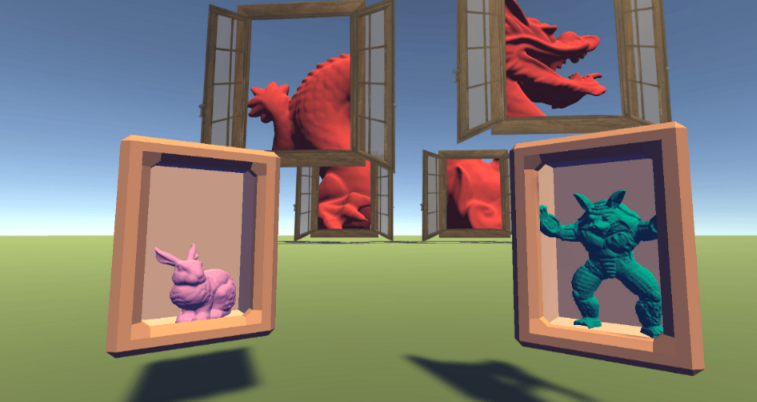
\includegraphics[width=12cm]{figuras/figura-7}}
	}{
		\Fonte{Ronja Tutorials (2021)}
	}
\end{figure}
\nocite{stcbuf}

Para suporte a visualização 3D estéreo, mais dois \textit{buffers} são utilizados em conjunto com os dois citados anteriormente para criar uma combinação com quatro \textit{buffers} de cor que são divididos para cada olho. Se um objeto 3D precisar ser desenhado com remoção de superfície encoberta, o \textit{buffer} de profundidade compara o valor da profundidade de cada \textit{pixel} dos objetos em cena para determinar qual será visível ou obscurecido. Há ainda a opção do uso de um \textit{stencil buffer} para aplicar operações complexas utilizando máscaras com o objetivo de determinar onde cada \textit{pixel} deve ser atualizado ou não \cite{GLSLBook}.

O \textit{buffer} de acumulação é capaz de reproduzir efeitos complexos como suavização em tela cheia de alta qualidade, profundidade de campo e desfoque de movimento. Ele funciona como um \textit{buffer} de cor, porém com maior precisão, capaz de acumular imagens para produzir uma úncia imagem composta. Já o \textit{multisample buffer} é capaz de produzir várias amostras da renderização para realizar suavização sem precisar renderizar a cena mais de uma vez. Por último, os \textit{buffers} auxiliares servem para guardar dados genéricos \cite{GLSLBook}. 

\subsubsection{Pipeline gráfica do OpenGL}
\label{sec:pipeline-opengl}

A máquina de estados do OpenGL possui uma ordem específica em que as operações do processo de renderização precisam ser realizadas. Essa padronização é chamada de \textit{pipeline} gráfica e é mostrada na Figura \ref{fig:pipeline}. Todos os dados necessários para desenhar a geometria estão contidos em espaço em memória e podem ser lidos pelo OpenGL de três maneiras diferentes \cite{GLSLBook}. 

\begin{figure}[h!]
	\centering
	\Caption{\label{fig:pipeline} \textit{Pipeline} gráfico do OpenGL.}	
	\UNIFORfig{}{
		\fbox{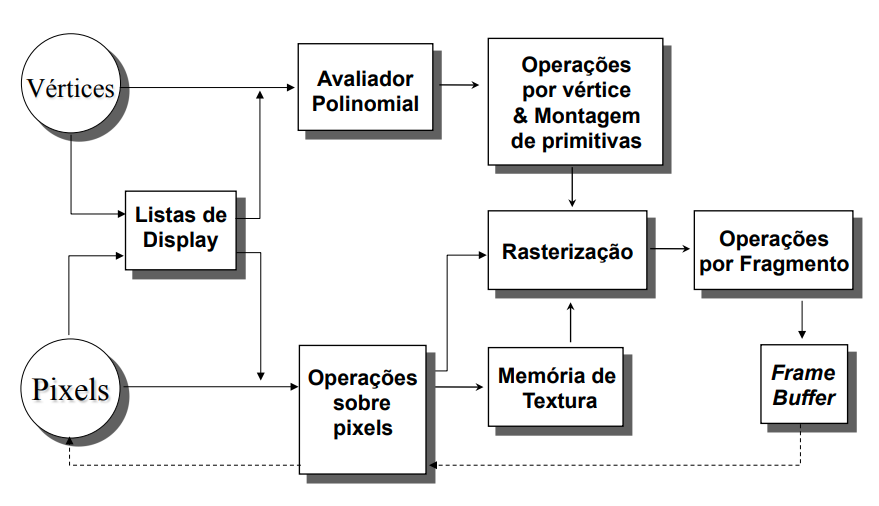
\includegraphics[width=11cm]{figuras/pipeline.png}}
	}{
		\Fonte{Montenegro (2021)} 
	}
\end{figure}
\nocite{pipeline}

A primeira maneira é enviar um vértice de cada vez utilizando comandos para manipular atributos dos vértices. A segunda é utilizar matrizes de vértices, o que oferece melhor performance devido a forma de organização dos dados, pois são utilizados ponteiros e mais dados podem ser processados de uma vez. Esses dois métodos fazem usam o modo imediato pois as primitivas são renderizadas assim que são especificadas. O terceiro método utiliza um dos dois procedimentos citados acima com uma lista de exibição --- uma estrutura de dados que guarda comandos para execução futura. Um ganho de performance desse método é a possibilidade de otimizar os comandos contidos na lista, ou ainda guardar os comandos na memória do acelerador gráfico \cite{GLSLBook}. 
	
A função do avaliador polinomial é derivar os vértices para conseguir representar superfícies e curvas. Isso é feito através do método de mapeamento polinomial, que produz as normais da superfície, as coordenadas da textura, as cores, e valores de coordenadas espaciais dos pontos de controle (VIEIRA, 2017)\nocite{pipelnRef}.

A próxima etapa é o estágio das operações por vértice que converte os vértices em primitivas. Alguns dados do vértice são transformados em matrizes de pontos flutuantes. Nesta etapa ocorre a projeção de coordenadas do espaço do mundo para o espaço da tela. Isso inclui algumas etapas como geração e transformação de coordenadas de textura, e também cálculos de luz para produção dos valores de cor (VIEIRA, 2017). Por isso é normal que essa etapa exija mais recursos computacionais. 

Logo em seguida ocorre a montagem das primitivas por meio do \textit{clipping} (eliminação de parte da geometria desnecessária para a renderização), que testa se a primitiva está totalmente dentro do plano de visualização, caso sim ela é repassada para o devido processamento. Caso ela esteja totalmente fora do plano de visualização ela é rejeitada. Se a primitiva estiver parcialmente visível no plano, ela é dividida para que somente a porção visível siga para processamento.

Outra operação desse estágio é a projeção das coordenadas da perspectiva para coordenadas da janela. Além disso, há uma etapa opcional de \textit{culling} onde os polígonos são testados para saber quais faces serão descartadas. Paralelamente a esse processo, os dados de \textit{pixels} contidos em uma matriz na memória do sistema são empacotados e processados por um mapa de pixels. Os artefatos resultantes podem ser escritos na memória da textura ou emitidos à etapa de rasterização \cite{GLSLBook}.

Rasterização é a etapa de conversão de dados tanto geométricos como de \textit{pixel} em fragmentos. Cada fragmento passa por algumas operações como: texturização; aplicação do valor de cor e profundidade; cálculos de névoa; testes de profundidade, transparência e remoção de faces ocultas (VIEIRA, 2017). Ao final são armazenados os valores no \textit{frame buffer}. Apesar de possuir muitos processos, é uma etapa simples e pode ser executada eficientemente para milhões de \textit{pixels} por segundo.

Na etapa de texturização a API tem capacidade de trabalhar com quatro tipos de texturas. Texturas de uma dimensão (vetor de pixels), texturas 2D (matriz $ mxn $ de pixels), texturas 3D, e mapas cúbicos. A API também pode trabalhar com formatos de imagem compactados, esses usam significativamente menos memória e melhoram a performance \cite{GLSLBook}.

É importante destacar que a API também fornece a possibilidade de utilizar texturas do tipo \textit{mipmap} --- várias representações da mesma imagem, porém cada uma tem metade da resolução da anterior --- em conjunto com o parâmetro de nível de detalhe que será detalhado mais adiante, mas que de forma simplificada permite a otimização do processo de renderização de objetos que estão distantes da câmera. 

Uma descrição matemática da \textit{pipeline} de renderização está na Equação \ref{eq-pipeline} onde $ (x, y) $ é a posição na tela de cada pixel, \textbf{v} é um conjunto de primitivas, $ p $ é o \textit{shader} de fragmentos, $ g $ é o \textit{shader} de geometria, $ h $ é o \textit{shader} de vértice e $ r $ é o estágio de rasterização onde as primitivas são convertidas em \textit{pixels} com atributos de geometria interpolados \cite{wang2014auto}.

\begin{equation} \label{eq-pipeline} \tag{1}
	\begin{aligned}
		f((x,y), \mathbf{v})=p \circ r(g \circ h(\mathbf{v}), (x,y)) 
	\end{aligned}
\end{equation}

Por fim, é importante mencionar que existem dois modos principais de renderização: o modo direto calcula as luzes e materiais para cada geometria visível e depois resolve qual está mais próxima da câmera para decidir quais exibir. Já o modo diferido realiza várias passadas para as geometrias e só então realiza os cálculos, dessa forma apenas os fragmentos visíveis são considerados. O segundo modo é mais eficiente para lidar com muitas luzes, porém não oferece suporte a transparência e suavização \cite{vsmid2017comparison}.

\subsubsection{Matrizes de transformação de coordenadas}
\label{sec:matrizes-transformacao-coordenadas}

Para o OpenGL transformar descrições de objetos tridimensionais em imagens 2D ele utiliza as informações do modelo do objeto, como posição dos vértices e normais da superfície, para interpretá-las como coordenadas do espaço do objeto. Como cada objeto tem suas próprias características, o sistema de coordenadas global é usado para que seja possível colocar vários objetos em uma única cena. Em seguida a API realiza mais uma conversão para o sistema de coordenadas de olho levando em consideração a posição e o ponto focal da câmera e o vetor de direção para cima \cite{GLSLBook}. 

Na equação \ref{eq-modelview}, a matriz \textit{modelView} é uma multiplicação das matrizes de conversão de coordenadas de espaço de objeto para espaço global e de espaço global para espaço de olho. O cálculo das normais é semelhante, a diferença é que é utilizada a matriz transposta da inversa da matriz \textit{modelView} para multiplicar um vetor de normais. 

\begin{equation} \label{eq-modelview} \tag{2}
	\begin{bmatrix}
		x_{olho} \\
		y_{olho} \\
		z_{olho} \\
		w_{olho} \\
	\end{bmatrix}
	=
	M_{modelView} \cdot
	\begin{bmatrix}
		x_{obj} \\
		y_{obj} \\
		z_{obj} \\
		w_{obj} \\
	\end{bmatrix}
\end{equation}

Como é possível ver na Figura \ref{fig:worldview} os três elementos mais à direita ($ m_{12} $, $ m_{13} $, $ m_{14} $) são para transformação de translação. O $ m_{15} $ é uma coordenada homogênea (Apêndice --- A) usada para transformação para o espaço de projeção. Os três conjunto de elementos ($ m_{0} $, $ m_{1} $, $ m_{2} $), ($ m_{4} $, $ m_{5} $, $ m_{6} $) e ($ m_{8} $, $ m_{9} $, $ m_{10} $) são usados para rotação e escala e representam os três eixos ortogonais x, y e z (AHN, 2021)\nocite{openglOnline}.

\begin{figure}[h!]
	\centering
	\Caption{\label{fig:worldview} Conteúdo das quatro colunas da matriz \textit{modelView}.}	
	\UNIFORfig{}{
		\fbox{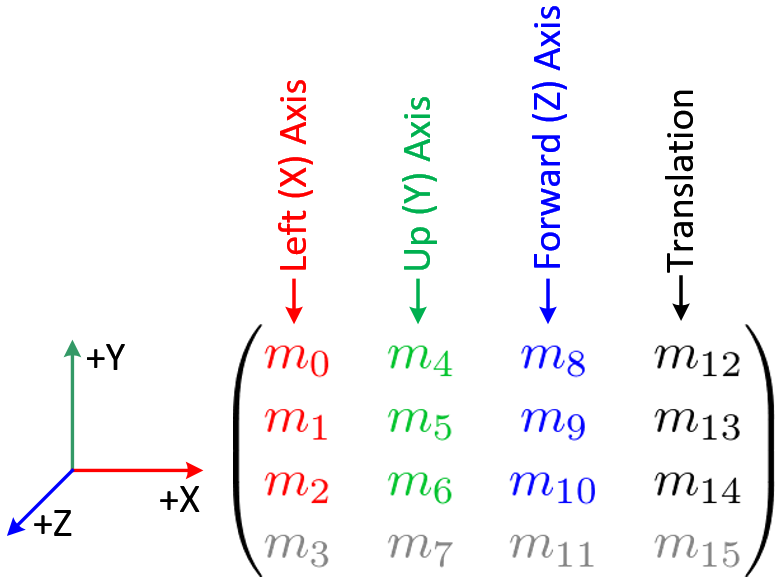
\includegraphics[width=6cm]{figuras/modelView.png}}
	}{
		\Fonte{Ahn (2021)}
	}
\end{figure}

Após essa conversão, as coordenadas obtidas são multiplicadas pela matriz de projeção para definir como os vértices serão projetados na tela, os valores dessa matriz dependem se modo de projeção utilizado é em perspectiva ou ortográfico (Figura \ref{fig:frustum}) e são mostrados nas equações \ref{eq-persp} e \ref{eq-ortho} respectivamente. 

\begin{figure}[h!]
	\centering
	\Caption{\label{fig:frustum} Modos de projeção de câmera. As letras correspondem a \textit{left, right, bottom, top, near e far}.}
	\begin{subfigure}{0.45\textwidth}
	\UNIFORfig{}{
		\fbox{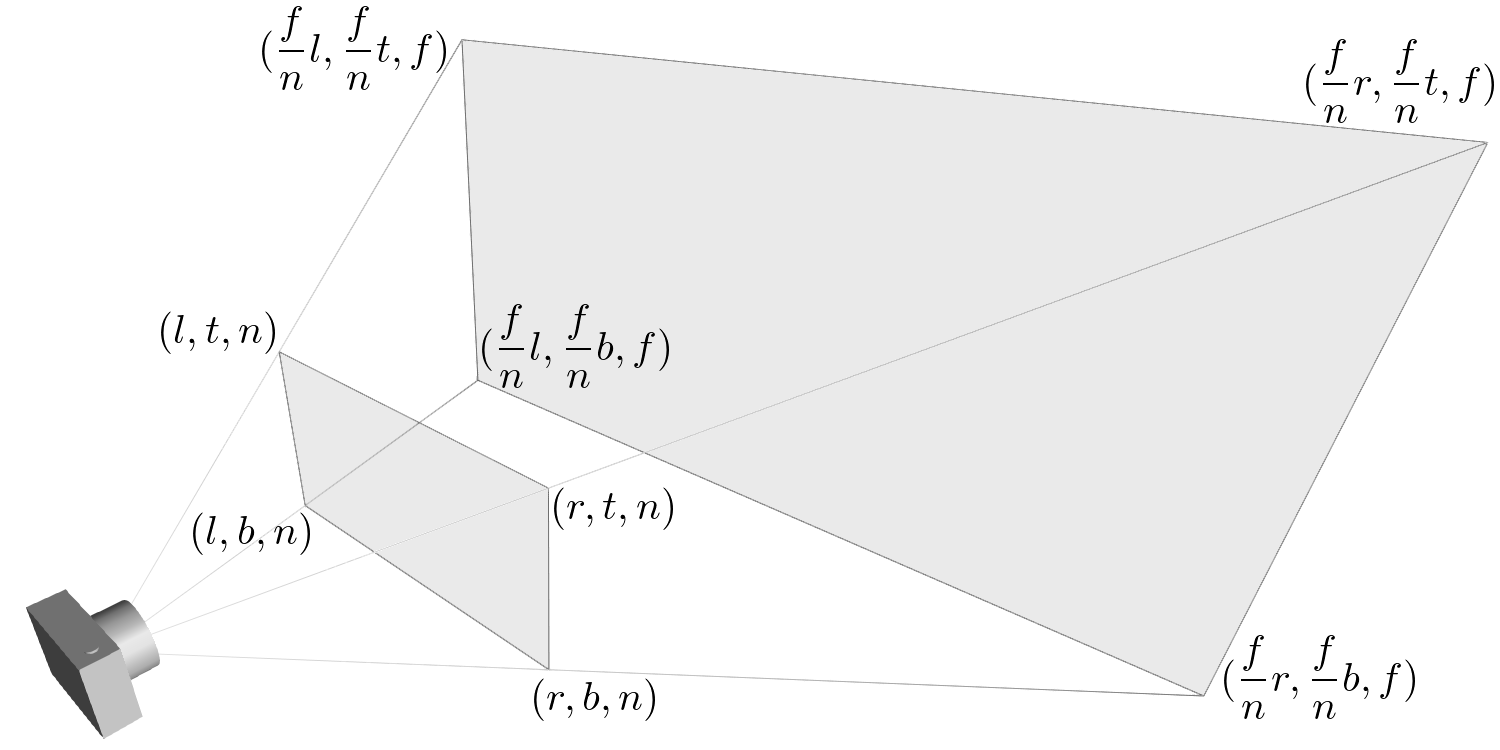
\includegraphics[width=\linewidth]{figuras/persp.png}}
	}{
		\caption{\Gls{view-frustum} em perspectiva}
	}
	\end{subfigure}
	\hfill
	\begin{subfigure}{0.47\textwidth}
	\UNIFORfig{}{
		\fbox{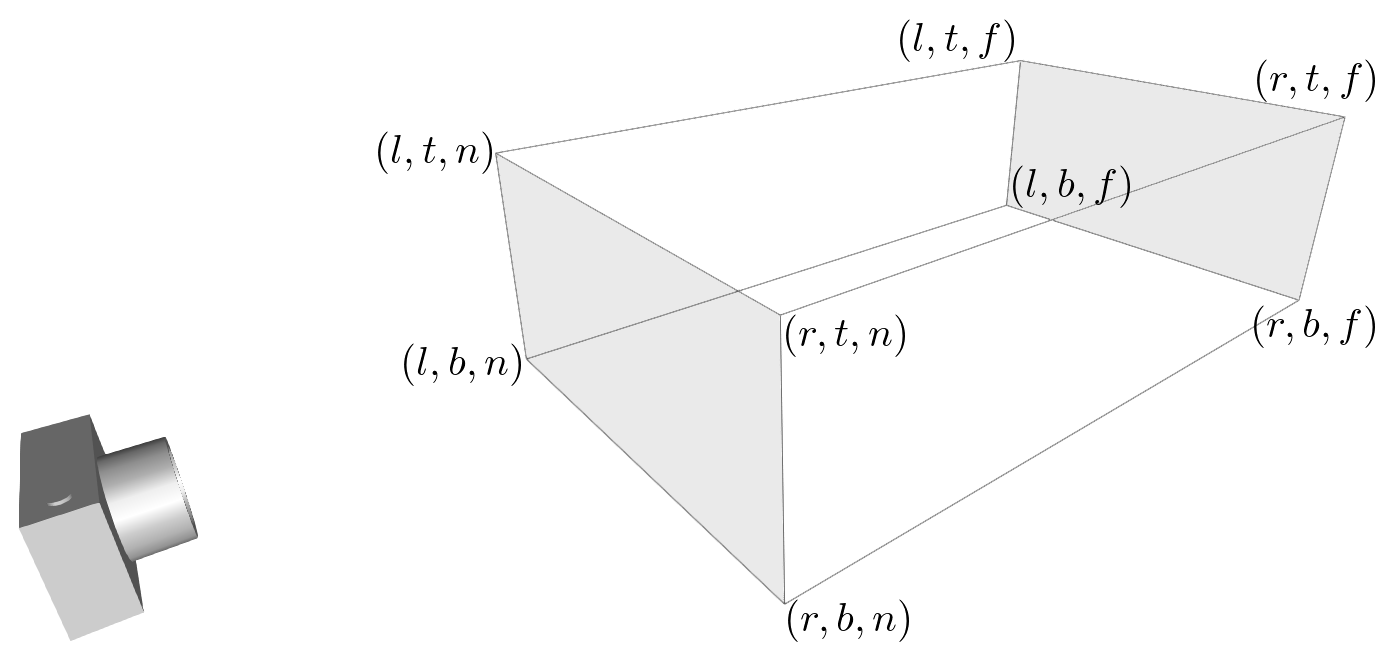
\includegraphics[width=\linewidth]{figuras/ortho.png}}
	}{
		\caption{\Gls{view-frustum} ortográfico}
	}
	\end{subfigure}
	{
		\Fonte{Ahn (2021)}
	}
\end{figure}

	\begin{equation} \label{eq-persp} \tag{3}
		\resizebox{.35\hsize}{!}{$ M_{persp}
		=
		\begin{bmatrix} 
			\cfrac{2n}{r-l} & 0 & \cfrac{r+l}{r-l} & 0 \\
			0 & \cfrac{2n}{t-b} & \cfrac{t+b}{t-b} & 0 \\
			0 & 0 & \cfrac{-(f+n)}{f-n} & \cfrac{-2fn}{f-n}\\
			0 & 0 & -1 & 0 \\
		\end{bmatrix} $}
	\end{equation}
	\begin{equation} \label{eq-ortho} \tag{4}
		\resizebox{.35\hsize}{!}{$ M_{orto}
		=
		\begin{bmatrix}
			\cfrac{2}{r-l} & 0 & 0 & -\cfrac{r+l}{r-l} \\
			0 & \cfrac{2}{t-b} & 0 & -\cfrac{t+b}{t-b} \\
			0 & 0 & \cfrac{-2}{f-n} & -\cfrac{f+n}{f-n}\\
			0 & 0 & 0 & 1 \\
		\end{bmatrix} $}
	\end{equation}

Os valores obtidos nessa operação são normalizados em uma região cúbica definida pelos pontos (-1, -1, -1) e (1, 1, 1) para espaço de coordenadas de dispositivo normalizado, ou seja, os valores passam a ser algum valor entre -1 e 1. Essa etapa é necessária para qua a área de visualização seja apropriadamente mapeada em uma janela de exibição de tamanho arbitrário. Por último, as coordenadas são convertidas para o sistema de coordenadas de tela. A partir desse ponto elas continuam para o processo de rasterização (AHN, 2021)\nocite{openglOnline}. 

\subsection{OpenGL Shading Language}
\label{sec:glsl}

Pela necessidade de substituir funcionalidades fixas por programabilidade em áreas que ficavam cada vez mais complexas (e.g. processamento de vértices e fragmentos) foram adicionados estágios programáveis por meio da introdução da linguagem de sombreamento \acrshort{GLSL}, feita para ser executada nos dois processadores programáveis existentes no OpenGL: o processador de vértices e o processador de fragmentos. Um \textit{shader} pode então ser definido como um código escrito em uma linguagem de sombreamento (HLSL, GLSL, RSL e etc) com o propósito de ser executado por um dos processadores programáveis do OpenGL. Um programa de \textit{shader} é então um conjunto de \textit{shaders} compilados executáveis \cite{GLSLBook}. 

A Figura \ref{fig:outline} mostra a implementação do código-fonte \ref{cf:outline} para criar um efeito de linha de contorno em volta de um objeto 3D utilizando a linguagem GLSL.

\phantom{a}

\phantom{a}

\begin{figure}[h!]
	\centering
	\Caption{\label{fig:outline} Demonstração de um \textit{shader} simples de linha contorno.}	
	\UNIFORfig{}{
		\fbox{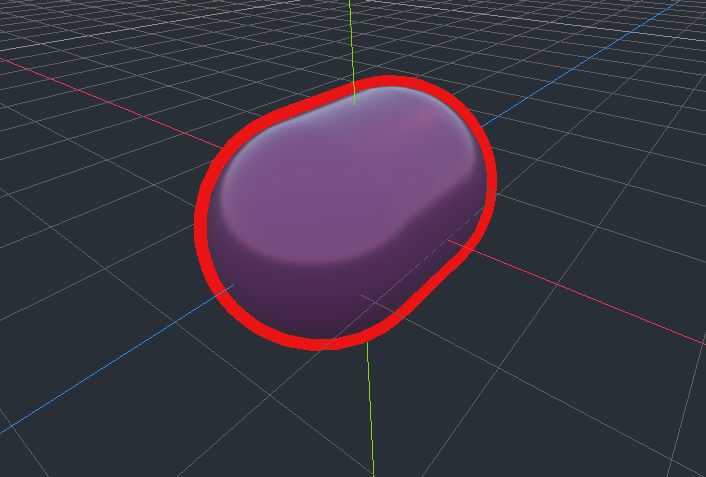
\includegraphics[width=8cm]{figuras/outline.png}}
	}{
		\Fonte{Elaborado pelo autor (2021)}
	}
\end{figure}

A linguagem GLSL faz uso de uma sintaxe similar a linguagem de programação C. Seus tipos incluem vetores e matrizes por serem estruturas fundamentais para cálculos matemáticos com operações para gráficos 3D. Os números de ponto flutuante (\textit{float}) também são fundamentais para conseguir altos níveis de precisão a troco de performance, por isso é possível especificar o nível de precisão ao utilizá-los. Além disso ela oferece suporte a laços, chamadas a sub-rotinas, expressões condicionais e possui funções embutidas \cite{GLSLBook}. 

Essa linguagem possibilitou aos desenvolvedores implementar um conjunto de diferentes técnicas para conseguir obter uma variedade de efeitos visuais; outrossim essas técnicas são implementadas com aceleração via \textit{hardware} pela GPU (com processamento paralelo) proporcionando um aumento drástico de performance e liberando carga da CPU para realizar outras tarefas.

O processador de vértices é uma unidade programável que realiza operações nos vértices e seus dados associados. Essas operações consistem em transformação de vértices, transformação e normalização das normais, geração e transformação das coordenadas de textura, iluminação e aplicação de cor. Variáveis de atributo são utilizadas para passar valores da aplicação para o processador de vértices. Já as variáveis uniformes são utilizadas para passar dados tanto para o processador de vértices como de fragmentos. Por último há as variáveis variantes cuja função é transportar informação do processador de vértices para o processador de fragmentos \cite{GLSLBook}.

O processador de vértices atua em um vértice por vez e uma implementação pode ter múltiplos processadores operando em paralelo. Logo, o \textit{shader} de vértice é executado uma vez para cada vértice, sendo que há uma possibilidade de perda de performance caso um \textit{shader} de vértice precise calcular mais variáveis variantes do que o que é necessário pelo \textit{shader} de fragmentos. Por outro lado, o processador de fragmentos é responsável por realizar algumas operações como interpolação de valores, acesso e aplicação de texturas, névoa e soma de cor \cite{GLSLBook}. 

Cabe ressaltar que, em termos de performance, normalmente os desenvolvedores preferem utilizar um \textit{shader} de vértice mais genérico em conjunto com um \textit{shader} de fragmento, pois assim é possível utilizar apenas um subconjunto das variáveis contidas no \textit{shader} de vértice e ainda sim reduzir tempo e custos de desenvolvimento e manutenção para uma grande quantidade de \textit{shaders} \cite{GLSLBook}.

\subsection{Direct3D \textit{versus} OpenGL}
\label{sec:direct-versus-opengl}

Direct3D é uma API para desenvolvimento de aplicações gráficas nativas para plataformas proprietárias da Microsoft. Ela evoluiu muito durante os anos 90 e superou a OpenGL. A \textit{pipeline} gráfica de ambas APIs são bem semelhantes, mas uma diferença importante se dá em termos de design de gerenciamento dos estágios de shaders, onde OpenGL faz uso de um objeto (programa de shader) que contém múltiplos \textit{shaders} enquanto que Direct3D expõe um contexto de renderização diretamente para a criação de \textit{shaders}. As linguagens GLSL e HLSL são muito parecidas e os desenvolvedores conseguem transcrever instruções facilmente de uma para a outra (MICROSOFT, 2021)\nocite{Direct3D}.

Essa interface faz parte da biblioteca de APIs do DirectX e é usada em consoles Xbox e sistemas Windows. DirectX também inclui algumas outras bibliotecas (e.g. Direct2D e DirectSound). Com o passar do tempo o foco voltou-se para APIs de acesso de baixo nível aos \textit{hardwares} gráficos como é o caso do DirectX 12. Entretanto sua versão anterior ainda é mais utilizada devido a questões de compatibilidade \cite{hasu2018modern}.

Devido a semelhança em capacidade de renderização entre as duas interfaces, a escolha sobre qual usar depende muito da plataforma alvo de desenvolvimento. Direct3D é específica para plataformas da Microsoft e é amplamente suportada por fornecedores de \textit{hardware} gráfico, especialmente em computadores \textit{desktop}. OpenGL é \textit{open source} e possui bastante aceitação no espaço de desenvolvimento \textit{mobile}, principalmente devido ao desenvolvimento da OpenGL ES --- uma subseção do OpenGL projetada especialmente para sistemas embarcados como \textit{smartphones} e consoles portáteis \cite{HLSLBook}.

Uma das principais diferenças é o ambiente de execução. O compilador HLSL traduz o código para linguagem de máquina que é processada pelo \textit{driver} do DirectX. Enquanto que no caso do OpenGL os fornecedores de \textit{hardware}, por serem responsáveis pela implementação do compilador, possuem muito mais liberdade para realizar otimizações em \textit{shaders}. Para mitigar essa diferença a Microsoft fornece uma solução (DirectX Effects Framework) para desenvolvedores elaborarem programas de \textit{shaders} iguais para \textit{hardwares} com menor ou maior capacidade de processamento \cite{GLSLBook}.

\subsection{High-Level \textit{Shader} Language}
\label{sec:hlsl}

Essa é uma linguagem de \textit{shader} criada em 2002 que também assemelha-se à linguagem C. Ao longo dos anos foram adicionadas melhorias como suporte a \textit{\Gls{multithread}}, adição de uma API para uso de GPGPU (\acrlong{GPGPU}) e suporte a tesselação. Na Figura \ref{fig:outlineHLSL} é mostrada a implementação de um \textit{shader} de contorno (ver código-fonte \ref{cf:outlineHLSL}) similar ao anterior para realçar as diferenças e semelhanças entre as duas linguagens.

\begin{figure}[h!]
	\centering
	\Caption{\label{fig:outlineHLSL} Efeito de contorno obtido com HLSL.}	
	\UNIFORfig{}{
		\fbox{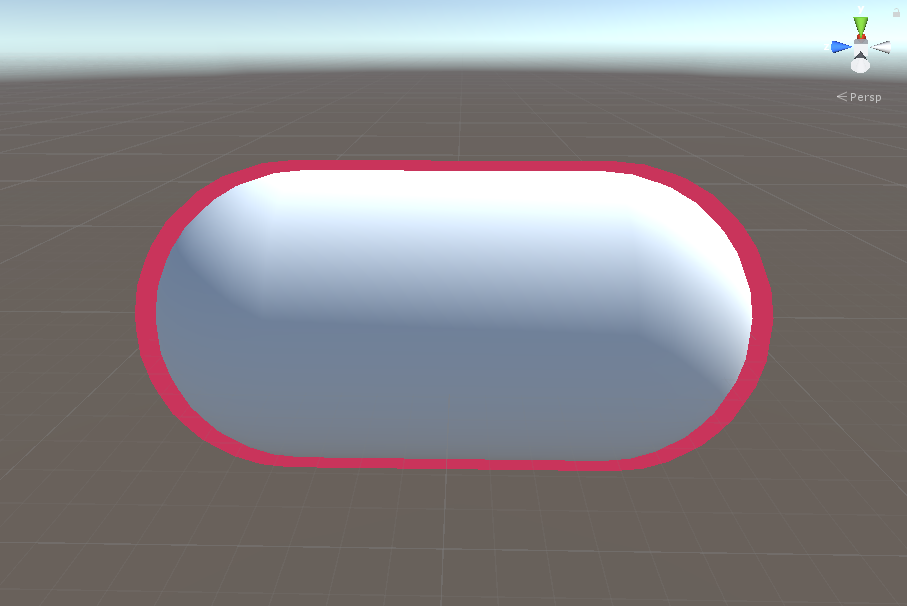
\includegraphics[width=7cm]{figuras/outlineUnity.PNG}}
	}{
		\Fonte{Elaborado pelo autor (2021)}
	}
\end{figure}

Uma GPU de propósito geral é uma unidade de processamento gráfico que realiza cálculos genéricos que normalmente seriam feitos pela CPU. São utilizadas para realizar tarefas custosas como cálculos de física, criptografia e computações científicas, pois é possível tirar proveito do paralelismo. Da mesma forma que um núcleo pode ser utilizado para renderizar múltiplos \textit{pixels} simultaneamente, ele também é capaz de processar múltiplos fluxos de dados ao mesmo tempo (TECHTARGET, 2021)\nocite{GPGPU}.

Tesselação é mais um processo na \textit{pipeline} gráfica responsável por adicionar detalhes a objetos diretamente pela GPU como mostrado na Figura \ref{fig:tess}. Seu modo de funcionamento consiste em subdividir um objeto dinamicamente e sem o custo adicional de reprocessamento de geometria. Isso permite um sistema de nível de detalhe dinâmico e menos utilização do barramento de gráficos, o que melhora a performance \cite{HLSLBook}.

\begin{figure}[h!]
	\centering
	\Caption{\label{fig:tess} Maiores níveis de tesselação produzem aumento no número de vértices.}	
	\UNIFORfig{}{
		\fbox{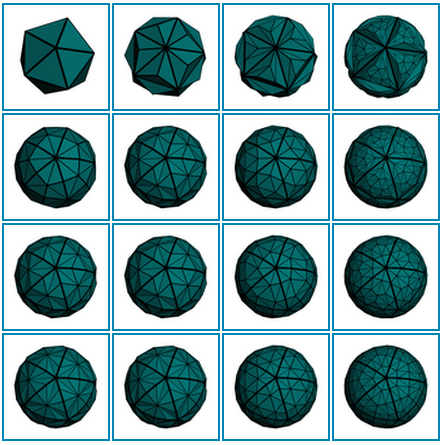
\includegraphics[width=6cm]{figuras/tess.png}}
	}{
		\Fonte{Wikimedia (2021)}
	}
\end{figure}
\nocite{tesselation}

Esse processo ocorre na etapa do \textit{shader} de geometria, que adiciona um passo de criação de geometria na \textit{pipeline} gráfica após o \textit{shader} de vértices. Isso permite que o programador implemente tesselação automática para geometrias complexas, ou realize operações gráficas dependentes de geometria como silhuetas e sombras \cite{bailey2007}.

Um \textit{shader} de geometria pode ter vários usos, por exemplo adicionar ou gerar mais primitivas (pontos, linhas, triângulos ou quadriláteros). Porém eles aceitam apenas uma quantidade limitada de topologias. Sua saída consiste em pontos, linhas ou triângulos e segue continuamente na pipeline. Basicamente, são utilizados os produtos dos \textit{shaders} de vértice e tesselação para montagem de primitvas \cite{hasu2018modern}.  

Shaders de tesselação interpolam geometria para acrescentar detalhes geométricos que permitem aos desenvolvedores realizar subdivisões adaptáveis, utilizar modelos mais "grosseiros" que serão refinados pela GPU, aplicar mapas de deslocamento detalhados sem fornecer detalhes de geometria, adaptar qualidade visual exigindo nível de detalhe e criar silhuetas suaves. Resumindo, tesselação é um processo que divide uma superfície em uma malha suavizada de triângulos e pode aumentar a qualidade da imagem final \cite{hasu2018modern}.

Eles possuem acesso a todas as informações na pipeline. São portanto capazes de escolher parâmetros de tesselação dinamicamente dependendo da informação lida. A principal diferença em relação aos \textit{shaders} de vértice é que enquanto esses modificam os vértices individualmente sem referência às primitivas, o \textit{shader} de tesselação amplifica uma única primitiva \cite{hasu2018modern}.

Nível de detalhe é um fator chave de otimização utilizado por \textit{game} \textit{engines} para alcançar renderização de alta qualiadade com melhor performance. Além disso é desejável evitar mudanças frequentes em \textit{shaders} e chamadas de desenho utilizando um número reduzido de shaders. Isso minimiza a sobrecarga da CPU e ajuda a GPU a desenhar mais objetos em um \textit{frame} com \textit{shaders} com nível de detalhe \cite{yong2015rapid}.

Em relação ao sistema de coordenadas, Direct3D faz uso do sistema de mão esquerda enquanto OpenGL utiliza o sistema de mão direita (Figura \ref{fig:direita}). Porém as aplicações são livres para utilizar seu próprio sistema de coordenadas. Um exemplo é o \textit{software} de modelagem 3D Blender que usa o sistema de mão direita, enquanto ambas Unity e Unreal utilizam o sistema de mão esquerda \cite{hasu2018modern}.

	\begin{figure}[h!]
		\centering
		\Caption{\label{fig:direita} Regra da mão direita.}	
		\UNIFORfig{}{
			\fbox{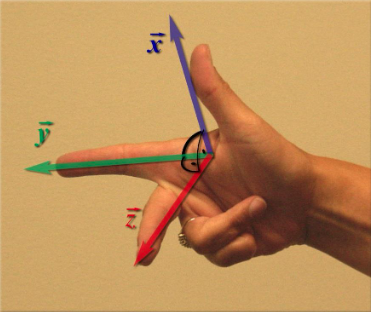
\includegraphics[width=6cm]{figuras/maoDireita.png}}
		}{
			\Fonte{Luiz (2021)}
		}
	\end{figure}
	\nocite{direita}

\section{Conceitos Técnicos de Shaders}
\label{sec:conceitos-tecnicos-shaders}

O HLSL é uma linguagem semelhante a C com estruturas extras para tratar vetores, matrizes e outros elementos relacionados a graficos. Com a melhoria da legíbilidade e da produtividade, os desenvolvedores podem focar no código e reutilizar otimizações de alto nível (como fazer uso de tipos correspondentes e funções embutidas). O compilador HLSL contém truques de otimização de baixo nível que podem ajudar \cite{riguer2002performance}.

Ao estudar computação gráfica a dúvida mais comum ao se deparar com os termos utilizados é "o que é um shader". Essa palavra pode causar uma certa estranheza no início mas sua definição não é tão complexa. Shaders são apenas pequenos programas (assim como um reprodutor de mídia ou uma calculadora de um computador) que são executados diretamente pela \acrshort{GPU} ao invés da \acrshort{CPU}. Isso permite a redução da carga de trabalho gráfico da \acrshort{CPU} pelo redirecionamento das tarefas para a \acrshort{GPU} que possui \textit{hardware} especializado para isso (LUTEN, 2021)\nocite{openGLBook}.

Um \textit{shader} computa alguns aspectos visuais de um objeto, como cor e deslocamento de superfície, tonalidade e direção da luz e efeitos volumétricos. São utilizados para especificar tranformações de vértices e cores de pixels. Pode-se pensá-los como uma função $ f $ que recebe um conjunto de valores $ v_i $ (como coordenadas de posição, normais e texturas) e um conjunto de parâmetros $ u_i $ (informação de cores e luz) e retorna a cor $ C_{xy} $ de cada objeto em cada \textit{pixel} $ xy $ da imagem final \cite{fabio2005user}. 

Shaders programáveis são uma das ferramentas mais impressionantes desenvolvidas para computação gráfica nos últimos anos. Através de seu uso, programadores ganharam flexibilidade para aplicar efeitos vértice-por-vértice e pixel-por-pixel com o processamento paralelo em gráficos interativos entre as mais diversas áreas como ciência, arte, engenharia, entre outras \cite{bailey2007}.

Um \textit{shader} contém um conjunto de instruções que são executadas concorrentemente para cada \textit{pixel} desenhado na tela. Essa forma de operação abre um leque de possibilidades, onde é possível por exemplo atribuir um comportamento para cada \textit{pixel} baseado na sua posição na tela. Em uma comparação com programação procedural, ele funcionaria como uma função que recebe uma posição e retorna uma cor, sendo que após a compilação seu tempo de execução é extremamente rápido (VIVO; LOWE, 2015)\nocite{bookOfShaders}.

É possível imaginar um \textit{shader} como um bloco de várias tarefas que passa por uma linha de produção industrial. As tarefas podem ser pequenas ou grandes e consequentemente podem demandar mais processamento e energia. No caso da CPU cada trabalho seguinte teria que esperar o término do atual para começar (VIVO; LOWE, 2015)\nocite{bookOfShaders}. É interessante ressaltar que hoje em dia existe a tecnologia de multiprocessamento, onde os computadores normalmente possuem grupos de quatro processadores que atuam em conjunto para realizar as tarefas.

Considerando uma tela com resolução de 800x600, significa que 480.000 \textit{pixels} precisam ser processados a cada \textit{frame} sendo que normalmente é utilizada uma taxa de 30 frames por segundo (\acrshort{FPS}), então será necessário fazer 14.400.000 cálculos por segundo. Isso explica o fato de video games e outras aplicações gráficas exigirem muito mais poder de processamento que outros programas. Seu conteúdo gráfico implica em inúmeras operações por cada pixel, pois cada \textit{pixel} na tela precisa ser computado (VIVO; LOWE, 2015)\nocite{bookOfShaders}.  

Esse cenário pode ser suficiente para sobrecarregar um microprocessador comum e fica pior quando leva-se em consideração as tecnologias que fazem uso seja de taxa de FPS maior, seja de resoluções maiores como 2K e acima. Para resolver esse problema utiliza-se processamento paralelo. A GPU possui vários pequenos microprocessadores que funcionam concorrentemente, além disso ela possui funções matemáticas específicas aceleradas via \textit{hardware} para realizar operações matriciais e trigonométricas rapidamente (VIVO; LOWE, 2015)\nocite{bookOfShaders}.

A dificuldade de programar \textit{shaders} levou ao desenvolvimento de ferramentas visuais que auxiliam a criação desses programas através do uso nós funcionais conectados entre si que remetem a uma estrutura de árvore. Esse tipo de ferramenta está presente na Unreal Engine desde 2005. Ao mesmo tempo que possuem utilidade, é importante garantir que \textit{shaders} gerados por tais ferramentas sejam otimizados. Otimização é importantíssima para encorajar desenvolvedores a criar \textit{shaders} maiores e mais complexos \cite{jensen2007shader}.

Conforme descrito em estudo por \citeauthoronline{wang2014auto} (2014) vários estudos sobre otimização de \textit{shaders} já foram conduzidos, porém com efetividade apenas para para o estágio de fragmentos. A qualidade dos \textit{shaders} depende bastante da experiência dos programadores e pode ser um processo bem demorado para níveis de complixadade maiores. Normalmente a computação mais custosa ocorre no \textit{shader} de fragmentos. 

Placas gráficas atuais oferecem suporte a quatro níveis de paralelismo: de dispositivo, de núcleo, de tarefa e de dados. O primeiro significa que vários processadores ou placas podem operar no mesmo sistema. O segundo significa que os múltiplos núcleos são independentes. O terceiro quer dizer que cada núcleo pode ter várias tarefas. Por fim, o quarto significa que múltiplas instruções podem agir em vários elementos de dados de uma vez \cite{hasu2018modern}.

Também é importante mencionar os \textit{shaders} de computação, que são um estágio fora da \textit{pipeline} de renderização utilizados para cálcular informações arbitrárias. São ótimos para implementar algoritmos que fazem uso da GPGPU. Podem também ser utilizados para acelerar partes da renderização. Suas entradas e saídas são genéricas e a única definição é do espaço de execução que é abstrato. Os dados processados são agrupados em grupos de trabalho (menor unidade de processamento) de tamanho definido pelo programador que são executados aleatoriamente e em paralelo \cite{hasu2018modern}.  

\subsection{Vertex Shader}
\label{vertex-shader}

Um \textit{shader} de vértice é um programa executado uma vez para cada vértice cujo é atribuído. As operações mais importante dessa etapa são as que envolvem cálculo de transformação e luzes. Dentre suas principais aplicações merecem destaque o suporte a criação de animações realistas e a possibilidade de deformar superfícies para criar efeitos realistas de ondas (NVIDIA, 2021)\nocite{vertexShader}.

O processador de vértices realiza as principais transformações de coordenadas descritas na Subseção \ref{sec:matrizes-transformacao-coordenadas}. Essa é uma ótima etapa para inserir código pois há bastante informação sobre a geometria. Quando essas coordenadas deixam o estágio de processamento, elas são cortadas e mapeadas para o sistema de coordenadas de tela, prontas para serem rasterizadas \cite{bailey2007}.

O \textit{shader} de vértices prepara o ambiente de \textit{shader} para o processamento de vértices, a tesselação e os \textit{shaders} de geometria e também para a rasterização e para o \textit{shader} de fragmentos. Aqui também podem ocorrer mudanças de coordenadas. Os dados recebidos são enviados para o estágio de processamento de vértices da \textit{pipeline} \cite{hasu2018modern}.

Podem ser passados coordenadas de vértice para o \textit{shader} de fragmentos utilizando geometria de espaço de objeto ou de olho. Por exemplo, para tesselação, o \textit{shader} de vértices pode passar primitivas conectadas com os dados que controlam a subdivisão que deve ser realizada, enquanto a saída do \textit{shader} de tesselação consiste em uma coleção de vértices para a nova geometria. No fim o principal objetivo de um \textit{shader} de vértice é pré-processar os vértices e gerenciar os atributos que seguirão para a \textit{pipeline} \cite{hasu2018modern}.

\subsection{Fragment Shader}
\label{sec:fragment-shader}

Um \textit{shader} de fragmento é um programa executado uma vez para cada pixel. Fragmentos são estruturas de dados contidas em cada \textit{pixel} que são criadas pela rasterização das primitivas. Um fragmento contém todos os dados necessários para atualizar seu espaço no \textit{frame buffer}. O processamento desses fragmentos consiste em operações feitas em cada pixel, sendo que as mais notáveis são a leitura da memória de textura e a aplicação do valor de textura para cada fragmento \cite{GLSLBook}. 

Nessa etapa o processador de fragmentos recebe as informações de cada pixel: seus valores de vermelho, verde, azul, transparência e coordenadas de textura. Cada \textit{pixel} também possui informação recebida do processador de vértices e interpolada na rasterização. Esse processador também pode acessar informações globais como a posição das luzes e seu trabalho final é processar essas informações e produzir a cor final de cada \textit{pixel} (ou descartá-lo). Sua grande utilidade consiste na possibilidade de customização da aparência dos \textit{pixels} de acordo com as necessidades do programador \cite{bailey2007}. 

Esse \textit{shader} é responsável por produzir a cor final para cada \textit{pixel} a partir de variáveis de estado e valores interpolados através de polígonos. Também é responsável por computar a cor e a intensidade da luz de cada fragmento. Além disso, é capaz de lidar com tipos diferentes de propriedades de vértices (os principais são coordenadas de textura e profundidade de pixels) \cite{hasu2018modern}. 

Dependendo da resolução definida, algo em torno de 2 milhões de \textit{pixels} podem precisar ser processados e renderizados a cada \textit{frame} (60 FPS). Isso facilmente gera uma carga computacional enorme. Felizmente, com a evolução da tecnologia, os desenvolvedores podem facilmente implementar programas que controlam a iluminação, o sombreamento e a cor de cada \textit{pixel} (NVIDIA, 2021)\nocite{fragShader}.

Shaders de fragmentos modernos são capazes de realizar centenas ou milhares de operações aritiméticas, incorporando funções trigonométricas custosas e vários acessos a mapas de textura para produzir a cor final de cada pixel. Consequentemente, seu custo de execução pode facilmente dominar a capacidade computacional por quadro \cite{lei2008acm}.

\section{Motores de jogo e suas ferramentas}
\label{sec:motores-jogo-ferramentas}

Um conjunto de ferramentas para criar um jogo é geralmente chamado de motor de jogo. Elas variam desde uma IDE (\acrlong{IDE}) até um pacote de \textit{software} com capacidade de simulação física, renderização, rede e inteligência artificial. Podem ser classificadas pelas dificuldade de uso, plataformas de destino ou gênero de jogo que podem criar \cite{compGameLang}. 

Sua principal função é ajudar os desenvolvedores oferecendo abstrações convenientes para os sistemas operacionais e seus \textit{hardwares} nos quais o jogo funcionará. Isso somado ao propósito de explorar ao máximo a capacidade das máquinas dos usuários para que seja proporcionada uma experiência mais imersiva possível \cite{simon2015unity}. O Quadro \ref{qua:engines} mostra alguns dos componentes mais importantes dos motores de jogo utilizados nesse estudo.

\begin{quadro}[h!]	
	\centering
	\Caption{\label{qua:engines} Principais componentes das \textit{game} \textit{engines}}\UNIFORqua{}{
		\begin{tabular}{|l|c|m{3cm}|c|}
			\hline
			\phantom{engines} & Godot & \centering Unity & Unreal \\
			\hline
			Shading & GLSL & \centering ShaderLab (HLSL) / \textit{Shader} Graph & Material Nodes \\
			\hline
			Sistema de Partículas & Built-in & \centering Built-in / VFX Graph & UnrealCascade\\
			\hline
			Motor de física & Bullet & \centering PhysX  & PhysX \\
			\hline
			Programação & GDSCript / C\# & \centering C\# & C++ / BluePrint \\
			\hline
			Audio & Bus System & \centering Audio Mixer & Sound Cue \\		
			\hline
		\end{tabular}
	}{
		\Fonte{Elaborado pelo autor (2021)}
	}
\end{quadro}


Conforme definido por Barczak, Woźniak (2019) motores de jogo são softwares (proprietários ou de código aberto) voltados para facilitar a criação de jogos eletrônicos. Seus sistemas permitem a integração de vários elementos como \textit{\Gls{scripts}}, malhas, animações e audios que juntos podem formar um jogo eletrônico que pode ser distribuído para diferentes plataformas por indivíduos ou companhias. 

Atualmente motores de jogo são utilizados não somente como ferramentas de desenvolvimento de jogos, mas também em comunidades científicas para estudos que envolvem simulações nas áreas de medicina, arquitetura (para design de ambientes), meteorologia, geologia (com simulação e estudo de topologias) e educação, principalmente através do uso de \Gls{realidade-virtual} e \Gls{realidade-aumentada} \cite{comparacaoDesempenho2}. 

Cada \textit{engine} conta com um motor de renderização com funcionalidades que facilitam o processamento das informações da cena (câmera, luzes, materiais e texturas). O Quadro \ref{qua:features} mostra os componentes de renderização dos motores utilizados nesse estudo. Esse motor é uma parte fundamental de uma \textit{game} \textit{engine} e consome a maior parte dos recursos. Como os jogadores esperam visuais melhores e os jogos precisam rodar em \textit{hardwares} inferiores, há um conflito que faz com que os motores de renderização precisem ser otimizados e configuráveis durante o desenvolvimento \cite{vsmid2017comparison}.

\begin{quadro}[h!]
	\Caption{\label{qua:features} Funcionalidades gráficas presentes nas game engines}\UNIFORqua{}{
	\begin{tabular}{|l|c|c|c|} \hline
		                          & Unity     & Unreal    & Godot     \\ \hline
		1. Texture                &           &           &           \\ \hline
		~1.1. Basic               & \ding{51} & \ding{51} & \ding{51} \\ \hline
		~1.2. Procedural          & \ding{51} & \ding{51} & \ding{51} \\ \hline
		2. Lighting               &           &           &           \\ \hline
		~2.1. Per-vertex          & \ding{51} & \ding{51} & \ding{51} \\ \hline
		~2.2. Per-pixel           & \ding{51} & \ding{51} & \ding{51} \\ \hline
		~2.3. Light Mapping       & \ding{51} & \ding{51} & \ding{51} \\ \hline
		~2.4. Gloss/Specular Maps & \ding{51} & \ding{51} & X         \\ \hline
		~2.5. Basic               & \ding{51} & \ding{51} & \ding{51} \\ \hline
		3. Shadows                &           &           &           \\ \hline
		~3.1. Shadow Mapping      & \ding{51} & \ding{51} & \ding{51} \\ \hline
		~3.2. Projected           & \ding{51} & \ding{51} & \ding{51} \\ \hline
	\end{tabular}
	}{
		\Fonte{Adaptado de \citeauthoronline{stelios2017} (2017)}
	}
\end{quadro}

Ambas as \textit{engines} Unity e Unreal contém um sistema de iluminação global que simula operação em tempo real. Boa parte dos cálculos de renderização de luz são feitos antes de exibir o primeiro \textit{frame} e seus resultados são utilizados durante a execução do jogo. As duas \textit{engines} oferecem suporte a sombreamento baseado na física (simulação da interação física entre as luzes e as superfícies). Além disso, destaca-se o suporte a algumas técnicas avançadas como suavização de bordas, reflexões em tempo real, oclusão de ambiente e profundidade de campo \cite{compStudyGE}. 

Em termos de qualidade de gráficos, Godot e Unity são considerados inferiores a Unreal, que é mais adequada para renderizar gráficos empolgantes e realistas. Sendo que Unreal Engine se destaca pelos seus notáveis efeitos de pós-processamento e por implementar um ótimo efeito de dispersão de subsuperfície mostrado na Figura \ref{fig:subsurface}.

\begin{figure}[h!]
	\centering
	\Caption{\label{fig:subsurface} A luz que penetra na superfície de um objeto translúcido é espalhada pela interação com o material e sai da superfície em um ponto diferente.}	
	\UNIFORfig{}{
		\fbox{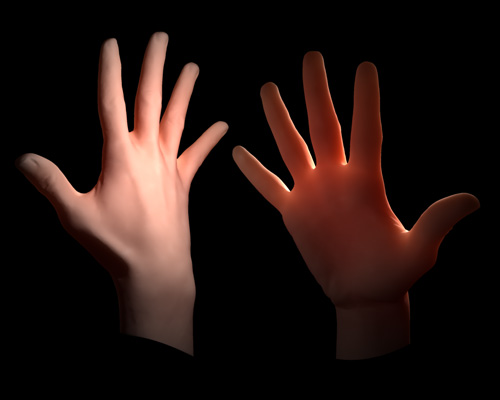
\includegraphics[width=9cm]{figuras/subsurface}}
	}{
		\Fonte{Mr Blue Summers (2021)}
	}
\end{figure}
\nocite{subsurface}

Para escolher qual dos motores de jogos será utilizado em um projeto é preciso ponderar alguns fatores como tipo de licensa, possibilidade de modificação do código, possível uso comercial, especificações de hardware, plataforma alvo, habilidade da equipe, ferramentas de suporte, estabilidade da \textit{engine} e público alvo \cite{navarro2012}.

Por serem ferramentas complexas, sua comparação é uma tarefa complicada. A maneira mais apropriada seria implementar o mesmo projeto com complexidade apropriada e de maneira similar em cada \textit{game} \textit{engine} utilizando critérios mensuráveis para avalização \cite{vsmid2017comparison}.  

\subsection{Godot}
\label{sec:godot}

Para Manzur e Marques (2018), Godot é uma \textit{engine} que difere arquiteturalmente em relação as outras duas \textit{engines}. Nesse caso cada sistema central é gerenciado por um servidor de forma assíncrona. Esses servidores operam em um alto nível de abstração. Apesar de soar complexo, sua interface é bem amigável. O sistema de árvore (Figura \ref{fig:gdtree}) de cenas permite organizar o conteúdo do jogo da forma que humanos estão acostumados a visualizar o mundo ao redor.

\begin{figure}[h!]
	\centering
	\Caption{\label{fig:gdtree} Estrutura hierárquica da cena na Godot Engine.}	
	\UNIFORfig{}{
		\fbox{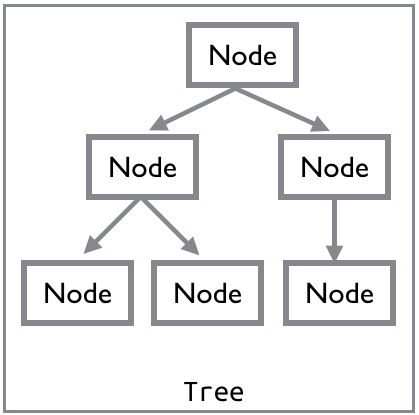
\includegraphics[width=7cm]{figuras/gdtree}}
	}{
		\Fonte{Packtpub (2021)}
	}
\end{figure}
\nocite{gdtree}

Todos os jogos criados nessa \textit{engines} são baseados no uso de nós e cenas. Nós podem ser considerados como átomos de funcionalidade de jogo e são utilizados em conjunto para formar cenas que podem ser combinadas para formar outras cenas mais complexas. Nós são parte fundamental dos jogos e consistem num bloco funcional com nome, propriedades e uma função especial. \cite{godotEngine}.

Uma funcionalidade que merece destaque é a de sinais, que são uma implementação do padrão de projeto de observador. O conceito básico é de que um objeto notifica outros objetos que possuem interesse em suas ações. O desenvolvedor não precisa se preocupar quando ou onde as ações serão solicitadas. Então o objeto emite o sinal e seus observadores são notificados \cite{godotEngine}.

\subsection{Unity}
\label{sec:unity}

Unity é um motor de jogo desenvolvido e mantido pela empresa Unity Technologies. Apesentada em 2005, sua primeira versão era simples e compatível apenas com Mac OS, porém com sua evolução foi adicionado suporte a outras plataformas (PC, Linux, Android, iOS, PS4, etc) \cite{compStudyGE}. Esse foi um dos principais fatores que tornou essa \textit{engine} tão popular.

Ela faz uso do DirectX como \textit{pipeline} de renderização padrão, mas além disso ela utiliza quatro atividades de renderização adicionais. A \textit{pipeline} de renderização direta é dividida em passagem de ambiente para objetos não afetados pela luz, passagem de transparência e passagem de luz para objetos opacos. Já a \textit{pipeline} de renderização diferida é baseada em um modelo inteligente que primeiro computa a geometria e depois aplica a luz \cite{simon2015unity}.

A \textit{pipeline} de renderização de pré-passagem é direcionada para as restrições no uso de diferentes \textit{shaders} no processo diferido. As informações de luz são guardadas em um \textit{buffer} para melhorar a performance dos cálculos. Por último é realizado o processo de renderização de vértices iluminados (cada objeto é renderizado com a iluminação de todas as fontes de luz calculada nos vértices) que é o mais rápido \cite{simon2015unity}. 

Apesar de sua \textit{pipeline} ser considerada uma caixa preta (desenvolvedores não possuem muito controle sobre seu funcionamento) por \citeauthoronline{hasu2018modern} (2018), há diferentes alternativas baseadas em renderização diferida, direta e legado (iluminação diferida ou por vértice). Cabe mencionar também a \textit{pipeline} de renderização programável que é uma forma alternativa de permitir que desenvolvedores configurem a renderização.

Há também a \textit{pipeline} de renderização de alta definição (\acrshort{HDRP}) voltada para computadores e consoles de última geração, que oferece iluminação coerente e unificada e melhores ferramentas de debug. Já a \textit{pipeline} peso-leve \acrshort{LWRP} é voltada para dispositivos móveis e realidade virtual que apresenta algumas otimizações de performance \cite{hasu2018modern}.

Sua arquitetura consiste em um sistema modular baseado em componentes que são utilizados para compor os objetos nos jogos. Cada componente possui um conjunto de funcionalidades que afetam o comportamento do objeto, dessa forma não é necessário usar herança. Isso é uma vantagem visto que aumenta a flexibilidade e a eficiência da modificação dos objetos \cite{compStudyGE}.

Cabe ainda destacar que ela possui uma das melhores documentações. A maioria das funções são descritas em profundidade e com bastante uso de exemplos, o que é muito útil principalmente para usuários iniciantes. Além disso ela possui uma vasta quantidade de templates, uma interface limpa e fácil de configurar, uma comunidade ativa, e seu uso de C\# ao invés de C++ torna a programação mais simples e agradável \cite{compStudyGE}.

Conforme verificado em estudo por Costa, Gomes, Duarte (2016)\nocite{estudoUnity}, dentre os motores de jogo a Unity é uma das ferramentas mais vantajosa do ponto de vista de produção por possuir um formato mais profissional e comercial, voltado para desenvolvimento multiplataforma. Além disso ela é capaz de performar melhor em composições de \textit{hardware} mais simples.

Apesar dos \textit{shaders} serem escritos na linguagem declarativa \textit{ShaderLab}, o código do programas é escrito como um \textit{snippet} HLSLPROGRAM que é transformado em código HLSL. Cada tipo de \textit{shader} é então definido usando a instrução \texttt{pragma}. Também há suporte para escrita manual de código GLSL, porém isso é recomendado apenas para testes ou casos específicos pois a Unity se encarrega de compilar e otimizar o HLSL para GLSL caso seja necessário para a plataforma alvo \cite{hasu2018modern}. 

Há ainda alguns \textit{shader} mais complexos que conseguem modificar a geometria base de malhas. São os \textit{shaders} de geometria e tesselação, que pode ser utilizados para adaptar a qualidade visual ao nível de detalhe exigido por meio da otimização da malha em tempo real conforme sua distância da câmera \cite{aino2020}.

\subsection{Unreal}
\label{sec:unreal}

Unreal, lançado em 1998, é um motor de jogo que também permite a criação de jogos para múltiplas plataformas. Ele possui uma ferramenta específica para criação de scripts chamada \textit{BluePrint} que permite implementar lógica de programação usando blocos, porém também é possível criar scripts em C++ \cite{compStudyGE}.

É uma \textit{engine} difícil de dominar por possuir excesso de opções à primeira vista, apesar de possui uma interface amigável. Seu sistema de programação com \textit{BluePrints} (Figura \ref{fig:blueprint}) traz uma vantagem para pessoas que não sabem ou não gostam de escrever código \cite{compStudyGE}.

\begin{figure}[h!]
	\centering
	\Caption{\label{fig:blueprint} A programação lógica e criação de materiais usa o sistema de \textit{BluePrint}.}	
	\UNIFORfig{}{
		\fbox{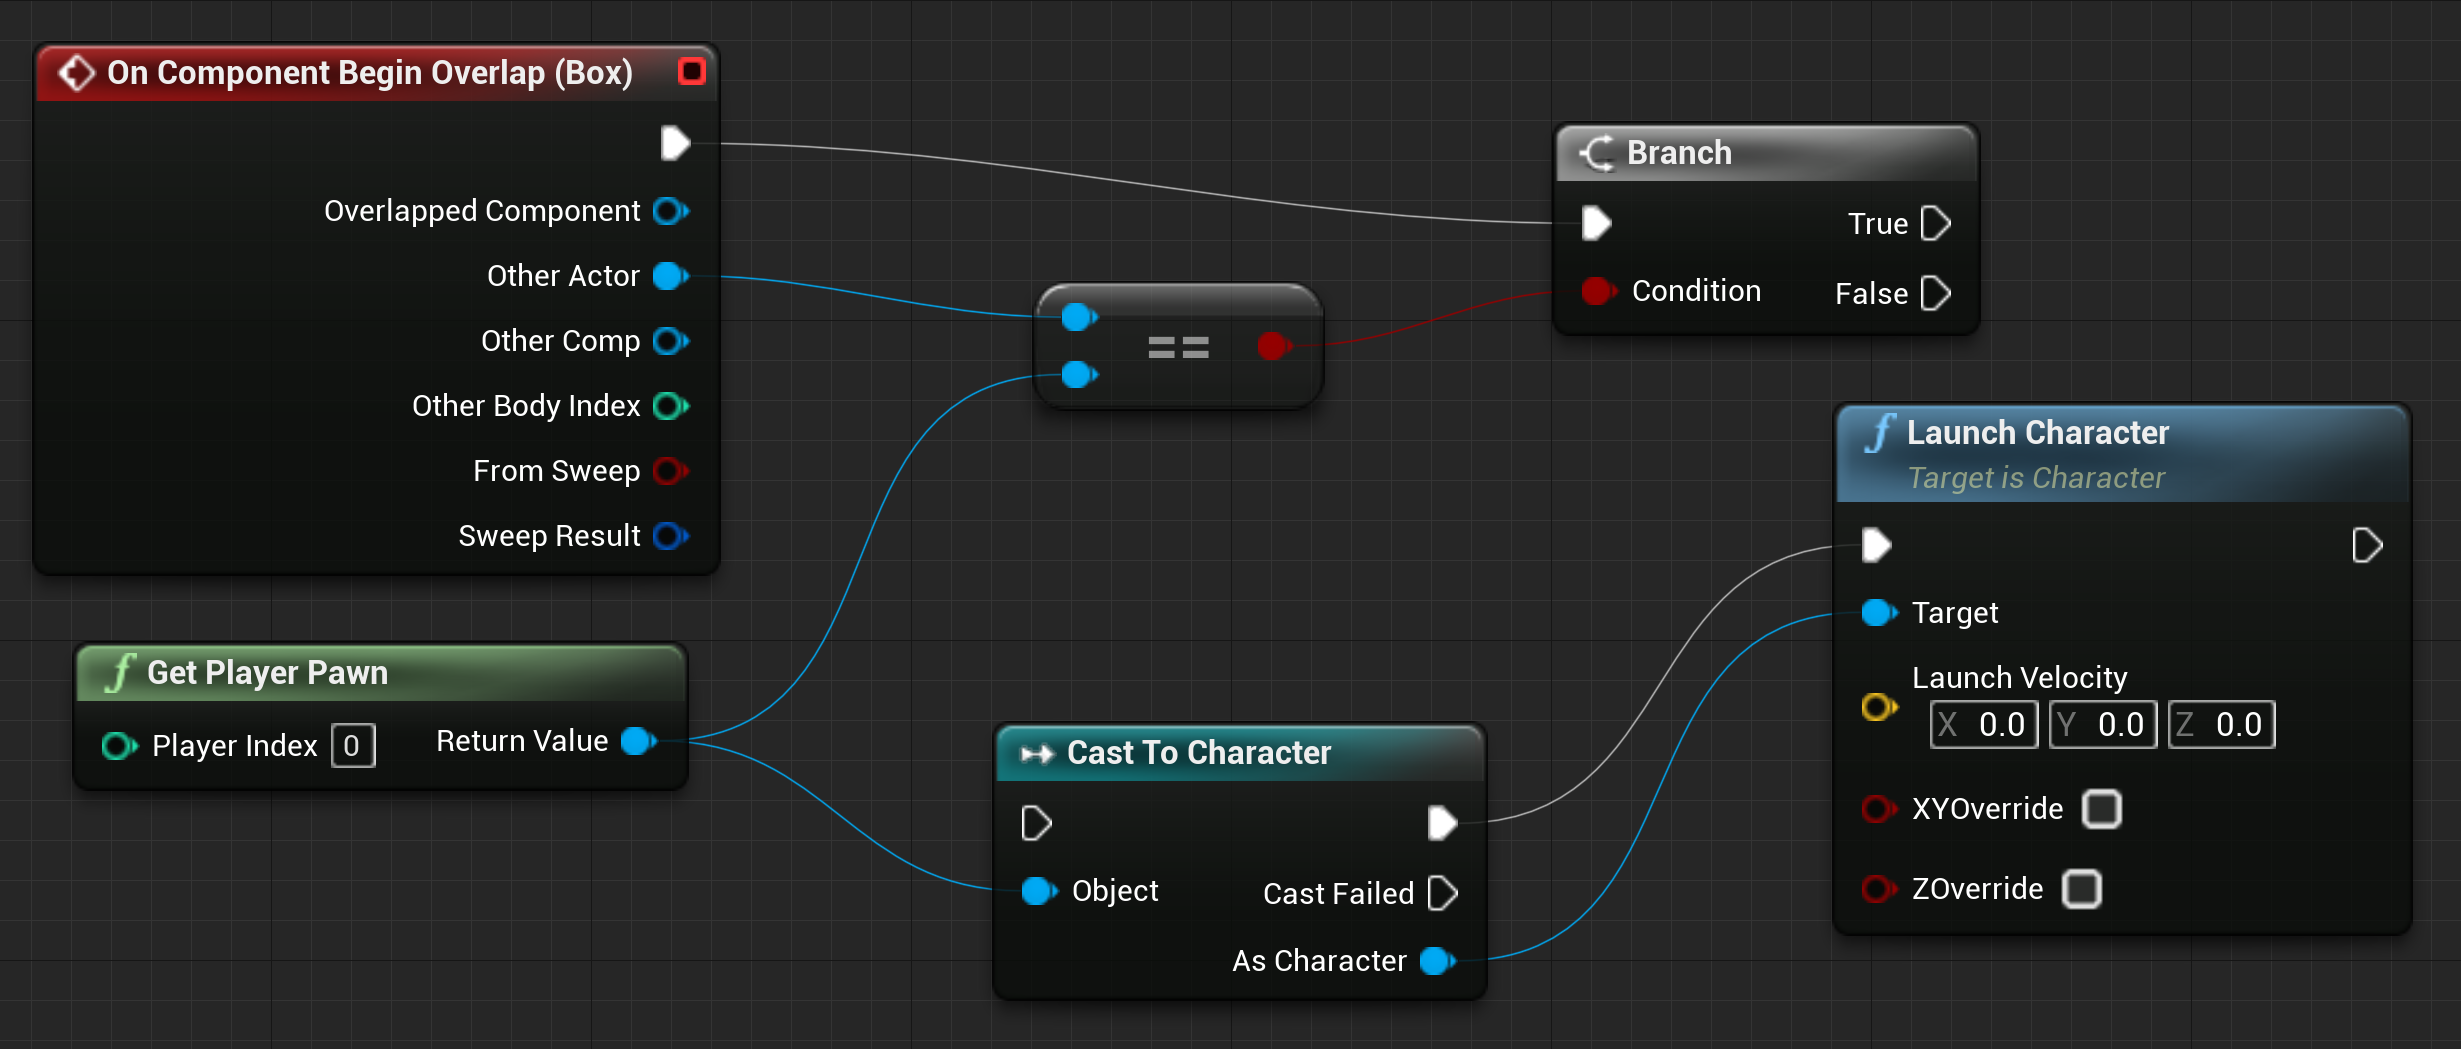
\includegraphics[width=13cm]{figuras/blueprint}}
	}{
		\Fonte{Unreal Engine (2021)}
	}
\end{figure}
\nocite{blueprint}

Merecem destaque seu sistema de renderização \Gls{multithread} (intitulado Gemini) com 64 bits de HDR (\acrlong{HDR}), oclusão de ambiente, iluminação por pixel, iluminação especular dinâmica e reflexões, seu sistema de customização de terrenos e ainda o sistema de malhas de navegação para integração com personagens controlados por inteligência artificial \cite{armstrong2013game}.

Unreal apresenta uma melhor performance audiovisual de maneira geral. Além disso ela apresenta uma interface mais complexa em comparação com Unity e Godot. É portanto uma \textit{engine} voltada para usuários mais experientes e \textit{hardwares} mais robustos \cite{stelios2017}.
 
\subsubsection{Nós de material}
\label{sec:material-nodes}

Unreal provê uma ferramenta de edição visual de grafos de nós para definição de expressões que computam parâmetros de entrada para modelos de materiais pré-definidos pela engine. Cada nó na expressão do grafo corresponde a um \textit{snippet} (pequeno pedaço de código) de \textit{shader} que é composto com código modelo de material provido pela própria \textit{engine} durante a compilação \cite{he2016rapid}.

Novamente a Unreal se destaca, por implementar uma ferramenta visual de edição de materiais que reutiliza os nós das \textit{BluePrints} mencionadas anteriormente, porém dessa vez voltadas para a modificação das propriedades dos materiais, o que torna o processo de criação de \textit{shader} bastante amigável e divertido por estimular visualmente a criatividade dos usuários \cite{compStudyGE}. 

Seu sistema de materiais é uma das melhores ferramentas. Para cada material é compilado um shader. Então é possível utilizar o mesmo material ou pequenas variações deste. Esse método proporciona aos artistas uma ferramenta poderosa para criação de materiais, porém o lado negativo é que no caso de \textit{shaders} mais complexos o tempo de compilação pode aumentar bastante \cite{vsmid2017comparison}.

Por baixo dos panos, essa \textit{engine} implementa uma otimização de sombreamento chamada cascata de sombras. Ela renderiza múltiplos mapas de sombra baseado na distância da câmera para que objetos mais próximos tenham sombras mais definidas que objetos distantes. Há uma mistura suave entre esses mapas para que a mudança seja quase imperceptível. Isso melhora a performance e é muito eficiente especialmente para grandes cenas \cite{vsmid2017comparison}. 

\section{Otimização e performance}
\label{sec:otimizacao-performance}

Embora as arquiteturas de \textit{shaders} forneçam execuções rápidas, a avaliação de \textit{shaders} gera um custo alto no processo de renderização. Shaders grandes (como os usados em filmes) podem igualar e exceder os custos associados com remoção de superfícies ocultas e processamento de geometria \cite{fabio2005user}. 

Isso torna-se um problema ainda maior em aplicações de tempo real que possuem restrições rígidas de taxa de quadros. Nesse caso, a simplificação geométrica é constantemente utilizada para fornecer um forma de compensação entre a qualidade da imagem percebida e a velocidade de execução em relação ao tamanho da malha do objeto \cite{fabio2005user}.

Cabe ressaltar que para \citeauthoronline{riguer2002performance} (2002), a performance média de um sistema é tão boa quanto o desempenho no pior gargalo. Então a tarefa de otimização pode ser reduzida à encontrar o pior gargalo e removê-lo (ou amenizá-lo). Esse é um processo iterativo que deve ser repetido até que o desempenho esteja em um limite aceitável.

Um gargalo de largura de banda de memória pode ocorrer quando há uso intenso de dados de vértices dinâmicos, uma solução seria reduzir a transferência de dados dinâmicos ou diminuir o tamanho de vértice. Já um gargalo de componente gráfico pode ser causado pelo próprio sistema \cite{riguer2002performance}.

O excesso de cálculos por vértice ou de uso de luzes pode causar um gargalo de processamento de vértices. Por outro lado, o uso de \textit{shaders} de fragmento complexos também pode gerar um gargalo. Além disso, o excesso de \textit{pixels} renderizados por segundo pode gerar um gargalo de taxa de preenchimento \cite{riguer2002performance}.

Outrossim, o uso de texturas de alta definição e de filtros complexos pode acarretar em um gargalo de carregamento de textura. Por fim, o uso excessivo de recursos de transparência, profundidade e amostragem pode causar um gargalo no processo de rasterização. Na maioria das vezes o que se percebe é uma combinação de vários gargalos atuando em conjunto \cite{riguer2002performance}. 

Usar geometria dinâmica é uma prática comum, porém não é bom abusar. Uma quantidade muito maior de polígonos pode ser obtida com geometria estática. Transformar geometria dinâmica em estática e aproveitar \textit{shaders} de vértice para mover animações para a GPU pode ajudar a balancear a carga de trabalho \cite{riguer2002performance}. 

Devido à sua natureza de operação em tempo real, os jogos eletrônicos são softwares que exigem bastante recursos de hardware. Principalmente quando os desenvolvedores cada vez mais objetivam criar produtos que perfaçam 60 frames por segundo (FPS) ou mais. Dessa forma, para atingir o maior público possível, vale a pena usar ferramentas que possibilitem o uso otimizado desses recursos \cite{comparacaoDesempenho}.

O crescimento do mercado de dispositivos móveis trouxe ampliou o desenvolvimento e a venda de aplicações sofisticadas para esses dispositivos. Entretanto há também uma enorme quantidade de desafios ao lidar com esse tipo de tecnologia, entre eles: fonte de alimentação, quantidade de poder computacional, tamanho do display e tipos de entrada \cite{optimizationMobile}.

Na GPU de dispositivos móveis o número de espaços de instrução é limitado para os \textit{shaders} de vértice e fragmento. Enquanto empacotar múltiplos ciclos de renderização em um único \textit{shader} de fragmento aumenta a contagem de instruções, aumentar a quantidade de ciclos de renderização diminui o fracionamento paralelo. Nesse caso a melhor solução dependerá das necessidades da aplicação \cite{designMobileGPU}. 

Segundo Singhal et al. (2011) algumas formas de otimizar \textit{shaders} seriam por meio de compressão de texturas para diminuir a sobrecarga de transferência de memória (ou utilizar um formato de \textit{pixel} de menor precisão), pré-computar coordenadas vizinhas de texturas no \textit{shader} de vértice e substituir laços por códigos otimizados ou utilizar vetores para realizar operações (diminuir a quantidade de instruções).

Considerando o trabalho de \citeauthoronline{nusrat2021commit} (2021), cabe aos desenvolvedores simplificar os gráficos para melhorar a performance. Simplificação de \textit{shaders} e de modelos 3D são os tipos de melhorias mais comuns que podem afetar a experiência visual dos usuários. Por exemplo, ativar o corte de oclusão estático/dinâmico desativa a renderização de objetos cobertos e ativar o \Gls{light-baking} pré-calcula efeitos de luz durante a compilação.

Nesse sentido, os desenvolvedores devem tentar entender o custo computacional dos \textit{shaders} e modelos 3D antes de usá-los. Para isso, antes de adicioná-los, devem ser feitos testes pois ao inserir vários modelos e \textit{shaders} pode ser difícil distinguir quais estão causando problemas de performance \cite{nusrat2021commit}.

Devido a melhoria no poder de processamento gráfico, o uso de técnicas como iluminação 3D, vegetação gerada proceduralmente e fotogrametria aumentou consideravelmente, tornando o processo de renderização mais custoso. Métodos comuns para otimização de cenas que fazem uso dessas técnicas são alocação de memória, \Gls{multithread}, e nível de detalhe. Ou seja, realizar a renderização em uma thread separada da lógica do jogo ajuda bastante a melhorar a performance \cite{zhang2017vegetation}.

Nível de detalhe determina a distribuição dos recursos de renderização entre os objetos de acordo com a posição e a importância atribuída aos vértices desses, diminuindo o número de dados desnecessários. Outrossim, são gerados modelos simplificados que reduzem a complexidade da cena e permitem uma renderização em tempo real mais eficiente \cite{zhang2017vegetation}.

Para \citeauthoronline{lewis2018evaluation} (2018), a quantidade de linhas de código de um \textit{shader} segue um distribuição de lei de potência, com poucos \textit{shaders} longos, e vários \textit{shaders} simples (poucas linhas). Entretanto, até os \textit{shaders} mais longos possuem em torno de 300 linhas. A maioria contém menos que 50 linhas. Isso mostra que normalmente \textit{shaders} são bem menores que softwares. A Tabela \ref{qua:instrucoes} mostra a contagem do número de instruções para operações de shaders.

\begin{table}[h!] 
	\centering
	\Caption{\label{qua:instrucoes} Número de instruções necessárias para operações específicas no OpenGL}\UNIFORqua{}{
	\begin{tabular}{|c|p{2cm}|p{2cm}||c|p{2cm}|p{2cm}|}
	\hline
	Operação & Número de Instruções & Número de ciclos de renderização & Operação & Número de Instruções & Número de ciclos de renderização \\
	\hline
	\begin{tabular}[c]{@{}c@{}}
		RGB2GRAY\\ RGB2YCbCr\\ YCbCr2RGB\\ RGB2HSV\\ HSV2RGB\\
	\end{tabular} &
	\multicolumn{1}{c|}{
	\begin{tabular}[c]{@{}c@{}}
		5\\ 14\\ 14\\ 28\\ 29\\
	\end{tabular}} &
	\multicolumn{1}{c||}{
	\begin{tabular}[c]{@{}c@{}}
		1\\ 1\\ 1\\ 1\\ 1\\
	\end{tabular}} &
	\begin{tabular}[c]{@{}c@{}}
		Gaussian \\Sharpening \\Gradient \\Bilateral \\Laplacian \\Box filter\\
	\end{tabular} &
	\multicolumn{1}{c|}{
	\begin{tabular}[c]{@{}c@{}}
		21\\ 13\\ 19\\ 62\\ 14\\18\\
	\end{tabular}} &
	\multicolumn{1}{c|}{
	\begin{tabular}[c]{@{}c@{}}
		1\\ 1\\ 2\\ 2\\ 1\\1\\
	\end{tabular}} \\
	\hline
	\begin{tabular}[c]{@{}c@{}}
		Bloom\\ Skin detection\\
	\end{tabular} &
	\multicolumn{1}{c|}{
	\begin{tabular}[c]{@{}c@{}}
		15\\ 25
	\end{tabular}} &
	\multicolumn{1}{c||}{
	\begin{tabular}[c]{@{}c@{}}
		1\\ 2
	\end{tabular}} &
	\multicolumn{1}{c|}{
	\begin{tabular}[c]{@{}c@{}}
		Sobel \\Prewitt
	\end{tabular}} &
	\multicolumn{1}{c|}{
	\begin{tabular}[c]{@{}c@{}}
		24\\ 16
	\end{tabular}} &
	\multicolumn{1}{c|}{
	\begin{tabular}[c]{@{}c@{}}
		2\\ 2
	\end{tabular}} \\
	\hline
	\begin{tabular}[c]{@{}c@{}}
		Detail enhancement \\Edge enhancement
	\end{tabular} &
	\multicolumn{1}{c|}{
	\begin{tabular}[c]{@{}c@{}}
		13\\ 25
	\end{tabular}} &
	\multicolumn{1}{c||}{
	\begin{tabular}[c]{@{}c@{}}
		1\\ 2
	\end{tabular}} &
	\multicolumn{1}{c|}{
	\begin{tabular}[c]{@{}c@{}}
		Contrast Stretching \\Median filtering
	\end{tabular}} &
	\multicolumn{1}{c|}{
	\begin{tabular}[c]{@{}c@{}}
		13\\ 43
	\end{tabular}} &
	\multicolumn{1}{c|}{
	\begin{tabular}[c]{@{}c@{}}
		1\\ 1
	\end{tabular}} \\ 
	\begin{tabular}[c]{@{}c@{}}
		Dilation \\Median
	\end{tabular} &
	\multicolumn{1}{c|}{
	\begin{tabular}[c]{@{}c@{}}
		22\\ 43
	\end{tabular}} &
	\multicolumn{1}{c||}{
	\begin{tabular}[c]{@{}c@{}}
		1\\ 1
	\end{tabular}} &
	\multicolumn{1}{c|}{
	\begin{tabular}[c]{@{}c@{}}
		Erosion \\Zero-crossing
	\end{tabular}} &
	\multicolumn{1}{c|}{
	\begin{tabular}[c]{@{}c@{}}
		22\\ 22
	\end{tabular}} &
	\multicolumn{1}{c|}{
	\begin{tabular}[c]{@{}c@{}}
		1\\ 1
	\end{tabular}} \\
	\hline
	\begin{tabular}[c]{@{}c@{}}
		Sepia \\Radial Blur \\Edge overlay \\Gray
	\end{tabular} &
	\multicolumn{1}{c|}{
	\begin{tabular}[c]{@{}c@{}}
		21\\ 21\\ 25\\ 5
	\end{tabular}} &
	\multicolumn{1}{c||}{
	\begin{tabular}[c]{@{}c@{}}
		1\\ 1\\ 2\\ 1
	\end{tabular}} &
	\multicolumn{1}{c|}{
	\begin{tabular}[c]{@{}c@{}}
		Color gradient\\Negative\\Gamma\\Edge
	\end{tabular}} &
	\multicolumn{1}{c|}{
	\begin{tabular}[c]{@{}c@{}}
		20\\ 2\\ 15\\ 24
	\end{tabular}} &
	\multicolumn{1}{c|}{
	\begin{tabular}[c]{@{}c@{}}
		1\\ 1\\ 1\\ 2
	\end{tabular}} \\ \hline  
	\end{tabular}
	}{
		\Fonte{\citeauthoronline{optimizationMobile} (2010)}
	}
	\end{table}

Como as GPUs normalmente possuem ótima capacidade de processamento de vértices, a etapa de sombreamento de vértices raramente gerará um gargalo. Entretanto quando muitos \textit{pixels} precisam ser processados por um \textit{shader} de fragmentos com muitas instruções é esperado que haja um gargalo. Pode-se dizer que o número de instruções é inversamente proporcional à performance (taxa de frames) \cite{optimizationMobile}.

O controle de precisão de ponto flutuante --- em OpenGL baixo (10 bits), médio (16 bits) e alto (32 bits) --- é uma ótima ferramenta para melhorar o desempenho, porém precisa ser usada de forma apropriada, pois um nível de baixa precisão apesar de melhorar a performance pode acabar gerando artefatos indesejados \cite{optimizationMobile}.

Além disso, como o número de vértices processados em operações de processamento de imagens é muito mais baixo que o de fragmentos, é recomendado realizar cálculos por vértice ao invés de por fragmento por aqueles serem menos custosos. Por fim, cabe salientar que maiores velocidades de clock favorecem a performance \cite{optimizationMobile}.

Como a criação de jogos tornou-se mais acessível, vários jogos são criados e lançados frequentemente. Com o aumento da quantidade de jogos no mercado os desenvolvedores precisam fazer com que eles se destaquem da concorrência. Para isso é comum o uso de modelos gráficos com muitos detalhes, o que pode acabar sobrecarregando o sistema significativamente \cite{performanceTesselation}. 

Quando muitos deles estão presentes na tela ao mesmo tempo, o jogo pode não funcionar bem, e isso afeta negativamente a experiência dos jogadores. Uma solução para esse problema consiste em aplicar algoritmos de tesselação para substituir dinamicamente modelos de objetos presentes no jogo. Cada modelo é substituído por um mais simplificado conforme a câmera se afasta, reduzindo a carga no sistema \cite{performanceTesselation}.

A maioria dos motores de jogos disponíveis no mercado oferecem uma ferramenta para geração automática de níveis de detalhe para modelos 3D. A única coisa que o desenvolvedor do jogo deve fazer é indicar como os níveis de detalhe devem ser gerados (caso os parâmetros padrões não se adequem ao projeto). A Unreal Engine possui uma ferramenta embutida para gerar níveis de detalhe por padrão com várias configurações prontas preparadas pelos criadores. A ferramenta é capaz de gerar automaticamente o número apropriado de níveis de detalhe \cite{performanceTesselation}.

Uma forma de otimização de \textit{shaders} já descrita por Rost (2006) consiste na substituição da função de ruído embutida na linguagem de \textit{shader} por uma função criada pelo próprio desenvolvedor ou por uma textura. A última opção é a melhor em termos de performance. Felizmente, a programabilidade oferecida pela GLSL torna possível pré-computar uma função de ruído e salvar seu resultado em mapas de textura de uma, duas ou três dimensões em cada um de seus quatro componentes.

Outra técnica útil para melhorar a performance ao lidar com várias luzes é o sombreamento diferido, que basicamente determina quais superfícies serão visíveis na cena final e aplica cálculos complexos de efeitos de \textit{shader} apenas nos \textit{pixels} que compõem essas superfícies. Dessa maneira, as operações são adiadas até que sejam estabelecidos os \textit{pixels} que contribuirão para a imagem final. Essa técnica garante que não haja desperdício de ciclos de \textit{hardware} com cálculos em \textit{pixels} que sequer serão exibidos na tela \cite{GLSLBook}.

Mais uma maneira de otimização descrita por Jensen \textit{et al}. (2007) seria garantir que o código de \textit{shader} seja movido para sua parte menos custosa. Nesse caso existem três possíveis lugares: no programa de vértices, no programa de fragmentos, ou nas declarações constantes. A última é a mais otimizada pois os cálculos são realizados em tempo de compilação. A segunda forma mais otimizada seria utilizar o espaço do programa de vértices, mas se houver muito código nessa parte haverá um desbalanceamento.

Caso seja necessário realizar transformações de coordenadas a melhor opção seria utilizar o espaço do programa de vértices, por exemplo mover transformação da direção da luz em espaço tangente para essa etapa. Ao ponderar-se esses detalhes para as ferramentas de criação de \textit{shaders} visuais, percebe-se que há uma certa dificuldade em realizar otimizações manuais, já que o código é gerado automaticamente \cite{jensen2007shader}.

Um dos erros mais comuns é usar texturas muito grandes desnecessariamente, o que prejudica bastante a performance, sendo que alguns objetos nunca atingem um tamanho grande na tela. O ideal seria tentar utilizar texturas com dimensões que não são potências de dois para diminuir o consumo de memória. Além disso, deve-se evitar a troca excessiva de texturas \cite{riguer2002performance}.

Segundo \citeauthoronline{arnau2014} (2014), uma possível técnica de otimização seria o uso de memoização para evitar a execução redundante de computações reutilizando resultados anteriores, o que resulta em aumento de velocidade de execução e economia de energia. De forma simplificada, os cálculos realizados são salvos em uma tabela para que no próximo cálculo os valores sejam reutilizados.

Para medir a performance, é necessária uma forma de \Gls{benchmark} para comparar a performance com mais precisão e objetividade. Alguma áreas onde o Benchmark é importante são na iluminação global, detecção de colisão, animação, renderização e em áreas onde é preciso medir e comparar a performance \cite{lext2001ray}.

Uma métrica muito comum para sistemas interativos de tempo real é a quantidade de quadros por segundo (taxa de quadros). Ela mede a frequência média de uma aplicação no \textit{hardware} onde é executada. Assim pode-se obter diferentes valores para diferentes tipos de hardware. Essa é uma medida comum entre várias revistas de jogos de computadores para medir a performance \cite{rehfeld2014profile}.

\citeauthoronline{he2016rapid} (2016) define o processo de otimização em várias etapas: identificação de componentes de \textit{shaders} que podem ser transformados em texturas, uso de pré-processamento \textit{offline} para os \textit{buffers} de parâmetros, seleção da melhor frequência espacial ou espaço de coordenadas para as funções e escolha de técnicas multi-resolução ou formas de reuso. Esse é um desafio enorme para motores de jogos modernos, que podem conter vários \textit{shaders} únicos, implementando uma vasta coleção de materiais e múltiplos níveis de detalhe que podem exigir diferentes procedimentos de otimização.
